%!TEX program = <xelatex>
\documentclass{pracamgr}
\usepackage{mystyle}
\usepackage{classDetails}

\begin{document}

	\setcounter{page}{1}
	\pagenumbering{roman}

	\maketitle
%\renewcommand\bibname{Spis literatury}	
	
	\begin{abstract}
Parallel Tempering (PT) is an extension to standard Metropolis-Hastings (MH) algorithm for simulating samples from a given distribution. The standard MH algorithm with high probability remains a local algorithm, in the sense that samples are drawn from some local probability mass cluster. This is highly problematic in case of multimodial distributions that frequently appear in applications, i.e. in bayesian hierarchical models. The PT algorithm is one of most celebrated possible solutions to that problem. 

Here we present a newly developed template for running simulations written in the R statistical programming language. Being highly modular it provides a general tool for performing simulations with many user provided state-spaces.
\end{abstract}

	\tableofcontents
	
	\addcontentsline{toc}{section}{List of figures}
	\listoffigures

	\addcontentsline{toc}{section}{List of tables}
	\listoftables

	\setcounter{page}{1}
	\pagenumbering{arabic}

	% Chapter
		% Section
		% Section
		% ...

	\chapter*{Introduction}
		\chapter*{Introduction}
\addcontentsline{toc}{chapter}{Introduction}


		
	\chapter{ Motivation }\label{motivation}	
		In this Chapter we motivate the use of the \PT\, making use of an example widely-cited in the literature,see \cite{BaragattiParallelTemperingWithEquiEnergyMoves} and \citet*{FamingLiang}. 

As pointed out in the Introduction, the reason for using the \PT\, is the multimodiality of the distribution of interest, $\pi$. In our simulations we assume to know the density function of $\pi$ to be the following mixture of normal densities:

\begin{equation}\label{experimental pi}
f(x) = 
\sum_{i=1}^{20} \frac{\omega_i}{ \sigma_i \sqrt{2 \pi} } \exp \Big( -\frac{(x - \mu_i)^\tran (x - \mu_i)}{2 \sigma_i^2} \Big),	
\end{equation}
where $\sigma_1 = \dots = \sigma_{20} = 0.1$, $\omega_1 = \dots = \omega_{20} = 0.05 $, and where  the means $\mu_i$ are given by

\begin{table}[ht]
	\centering
\begin{tabular}{rrrrrrrrrr}
  \hline
$\mu_1$ & $\mu_2$ & $\mu_3$ & $\mu_4$ & $\mu_5$ & $\mu_6$ & $\mu_7$ & $\mu_8$ & $\mu_9$ & $\mu_{10}$ \\ 
  \hline
2.18 & 8.67 & 4.24 & 8.41 & 3.93 & 3.25 & 1.70 & 4.59 & 6.91 & 6.87 \\ 
  5.76 & 9.59 & 8.48 & 1.68 & 8.82 & 3.47 & 0.50 & 5.60 & 5.81 & 5.40 \\ 
   \hline
\end{tabular}
\end{table}
and 

\begin{table}[ht]
	\centering
\begin{tabular}{rrrrrrrrrr}
  \hline
$\mu_{11}$ & $\mu_{12}$ & $\mu_{13}$ & $\mu_{14}$ & $\mu_{15}$ & $\mu_{16}$ & $\mu_{17}$ & $\mu_{18}$ & $\mu_{19}$ & $\mu_{20}$ \\ 
  \hline
5.41 & 2.70 & 4.98 & 1.14 & 8.33 & 4.93 & 1.83 & 2.26 & 5.54 & 1.69 \\ 
  2.65 & 7.88 & 3.70 & 2.39 & 9.50 & 1.50 & 0.09 & 0.31 & 6.86 & 8.11 \\ 
   \hline
\end{tabular}
\end{table}
 
Figure \ref{ToyExample} inspects visually the density. One notices easily that different peaks get intermingled, as only $15$ out of $20$ peaks are clearly visible.  

\begin{figure}
	\begin{minipage}[b]{.5\linewidth}
		\centering 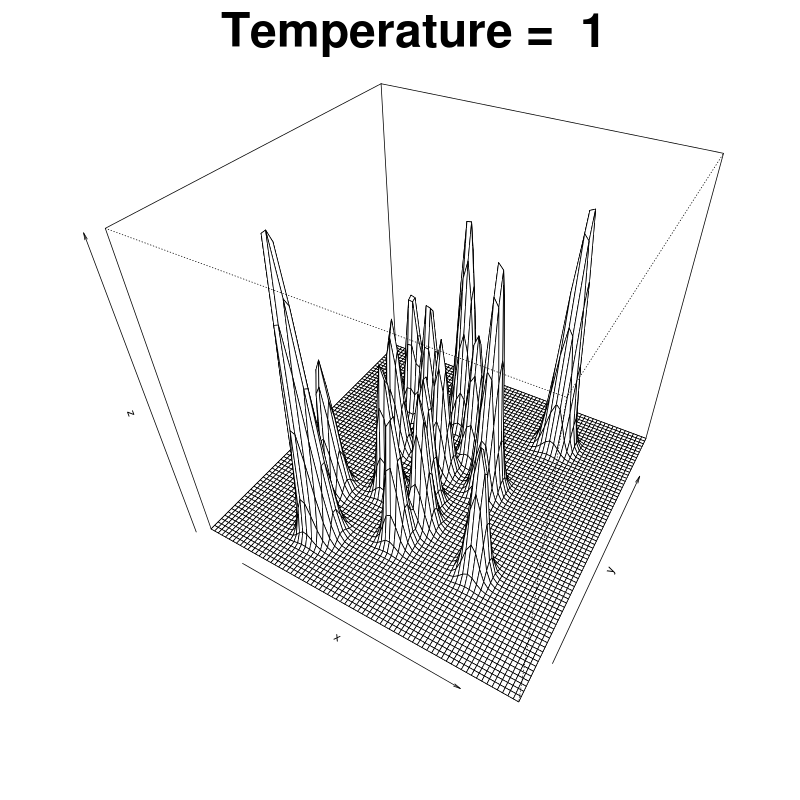
\includegraphics[scale=.25]{./img/Liang_perspective.png}
		\subcaption{Perspective view}\label{LiangContour}
	\end{minipage}%
	\begin{minipage}[b]{.5\linewidth}
		\centering 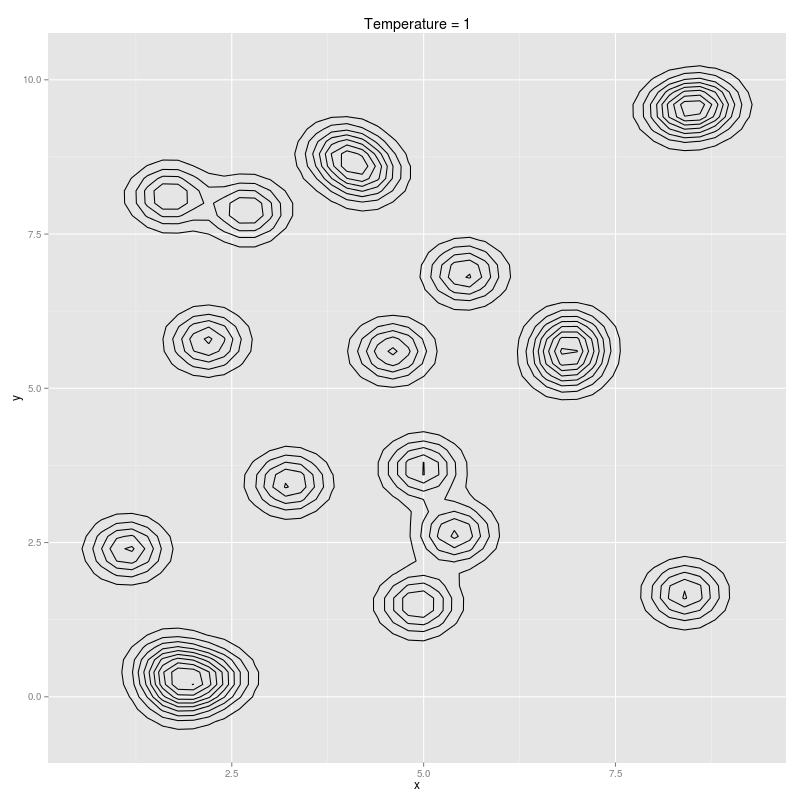
\includegraphics[scale=.25]{./img/Liang_Contour_plot.png}
	\subcaption{Level-set view}\label{LiangPerspective}
	\end{minipage}
	\caption{Toy-example density.}\label{ToyExample}
\end{figure}

The \MH\, is known to be a local algorithm and the reasons for it will be exposed in Chapter \ref{theory}. To motivate the use of the \PT\, it is enough to say for now that sample points generated by the usual \MH\footnote{For introduction to the theory behind the Metropolis-Hastings algorithm consider \cite{CharlesJ.Geyer}.} will be more often drawn from the vicinity of modes. This in turn might give the impression that most of the probability is concentrated somewhere next to the starting points\footnote{We choose the starting points at random}. We shall refer to the percentages of iterations in the vicinity of a particular mode its sojourn time, without giving its full definition right now.

In theory, by the ergodic theory, the sojourn times for each mode should converge to the probabilities of the modes' vicinity areas. However, in practical terms, this convergence might be prohibitively long, especially to what a typical user would consider to be a fortunate amount of computation time. This is clearly a big problem, since in practical applications, as mentioned in the Introduction, one considers the approximation of the needed integral to be simply the mean evaluation of a function on the generated sample point and these approximations cannot possibly be good if we cut the procedures too quickly. 

To investigate the \MH's localness, we have run the \Metro\, routine choosing the \sspace\, to be \realTemp. Figures \ref{unexploredShort} and \ref{unexploredLong} show that the localness of the algorithm is persistent even with longer runs of the \MH.  

\begin{figure}
	\begin{minipage}[b]{.5\linewidth}
		\centering 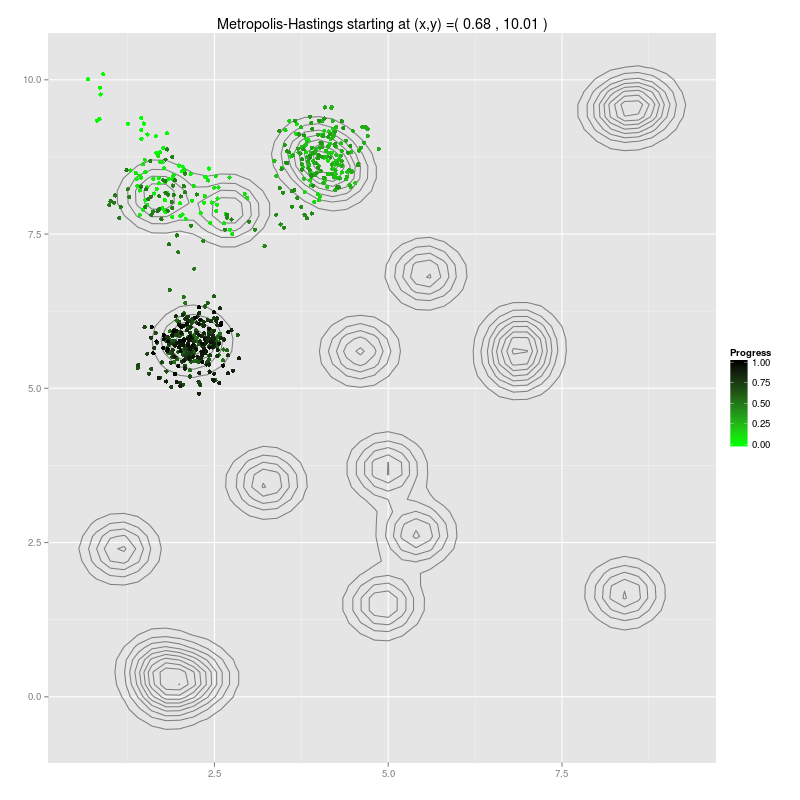
\includegraphics[scale=.25]{./img/MH_simululation_1000_steps_ex1.png}
		\subcaption{Thousand steps\dots}
	\end{minipage}%
	\begin{minipage}[b]{.5\linewidth}
		\centering 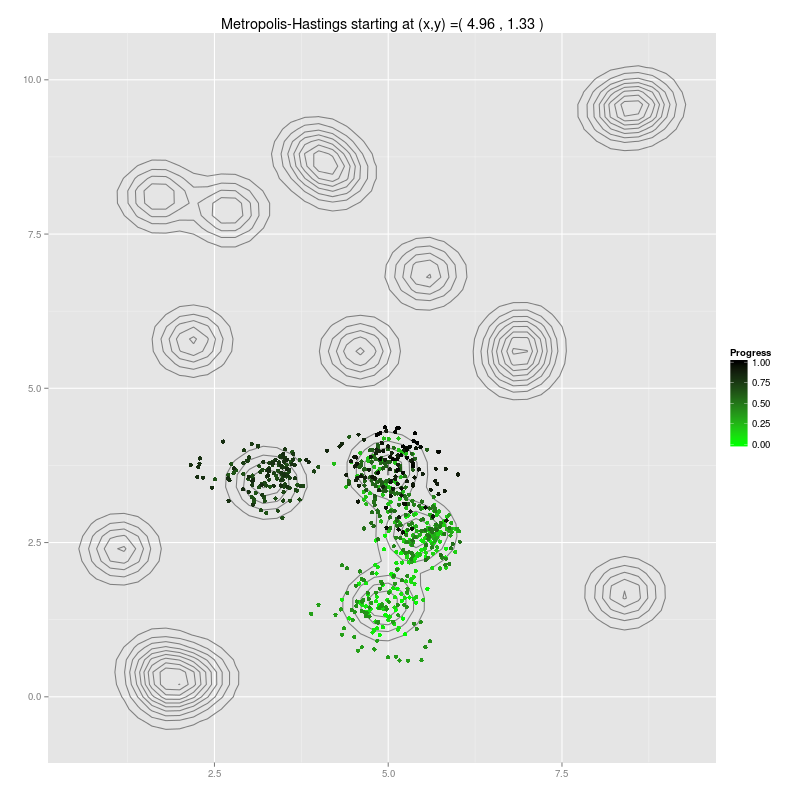
\includegraphics[scale=.25]{./img/MH_simululation_1000_steps_ex2.png}
	\subcaption{\dots that lead nowhere.}
	\end{minipage}
	\caption{Thousand Iterations - about $250$ different points generated. Colour intensity increases as points get generated in more advanced stages of the algorithm. One notices easily that short runs of the algorithm do not explore the whole \sspace.}\label{unexploredShort}
\end{figure}


\begin{figure}[ht]
	\centering 
	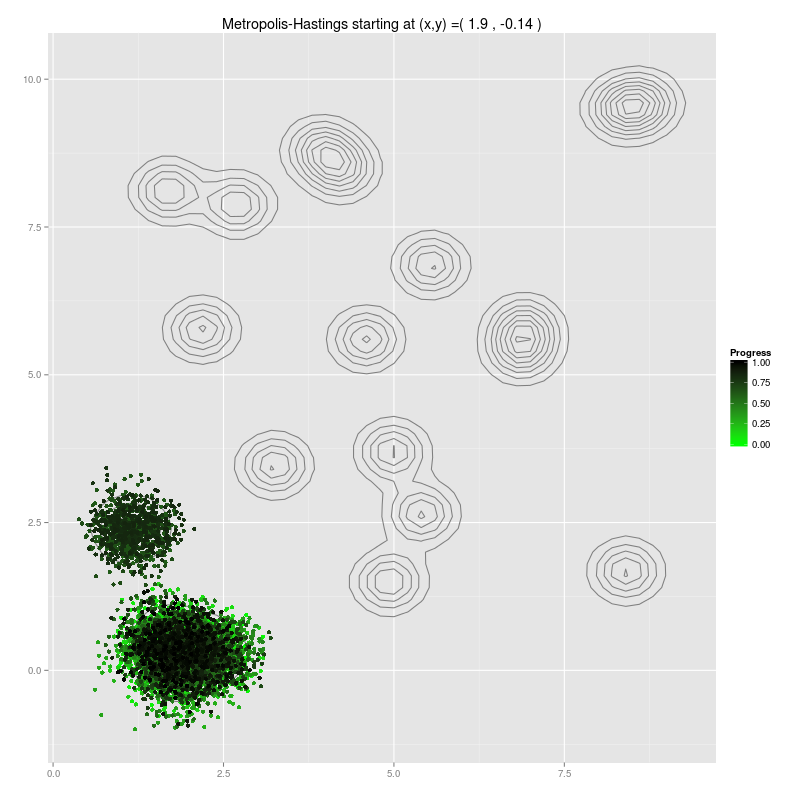
\includegraphics[width=\textwidth,keepaspectratio]{./img/MH_simululation_10000_steps.png}
	\caption{Ten Thousand Iterations - about a quarter of which resulted in different points. Again the \MH\, failed at exploring the whole \sspace.}\label{unexploredLong}
\end{figure}

Everything changes when one considers the \PT\, instead, as seen in Figures \ref{PTshort} and \ref{PTlong}.

\begin{figure}
	\begin{minipage}[b]{.5\linewidth}
		\centering 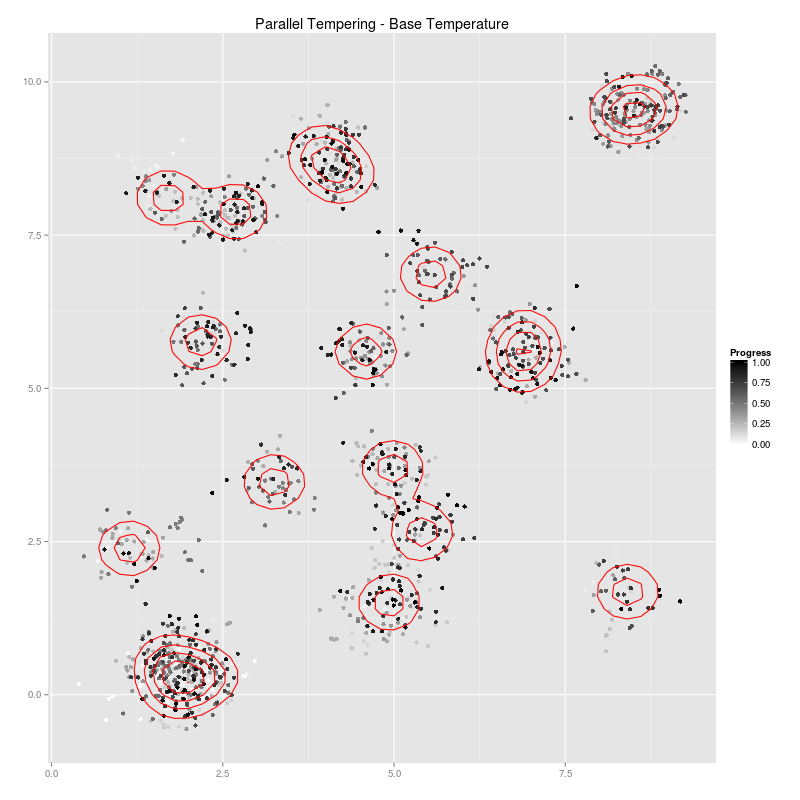
\includegraphics[scale=.25]{./img/PT_simululation_base_temperature_2000_steps_strategy_1_try_1.png}
		\subcaption{Two thousand steps\dots}
	\end{minipage}%
	\begin{minipage}[b]{.5\linewidth}
		\centering 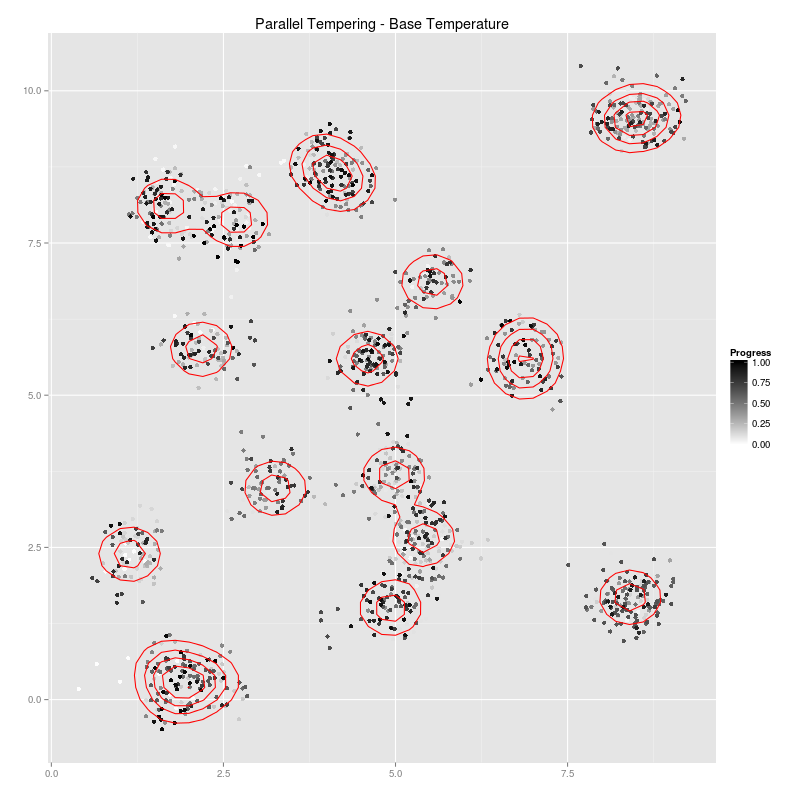
\includegraphics[scale=.25]{./img/PT_simululation_base_temperature_2000_steps_strategy_2_try_1.png}
	\subcaption{\dots that always lead to Rome.}
	\end{minipage}
	\caption{Results of the \PT\,when \strat\,1 and \strat\,2 from Chapter \ref{theory} are applied. One notices immediately the qualitative difference between these examples and the \MH\,results, as the \sspace is explored more thouroughly. The results are obtainable under a minute on a modern computer.}\label{PTshort}
\end{figure}

\begin{figure}[ht]
	\centering 
	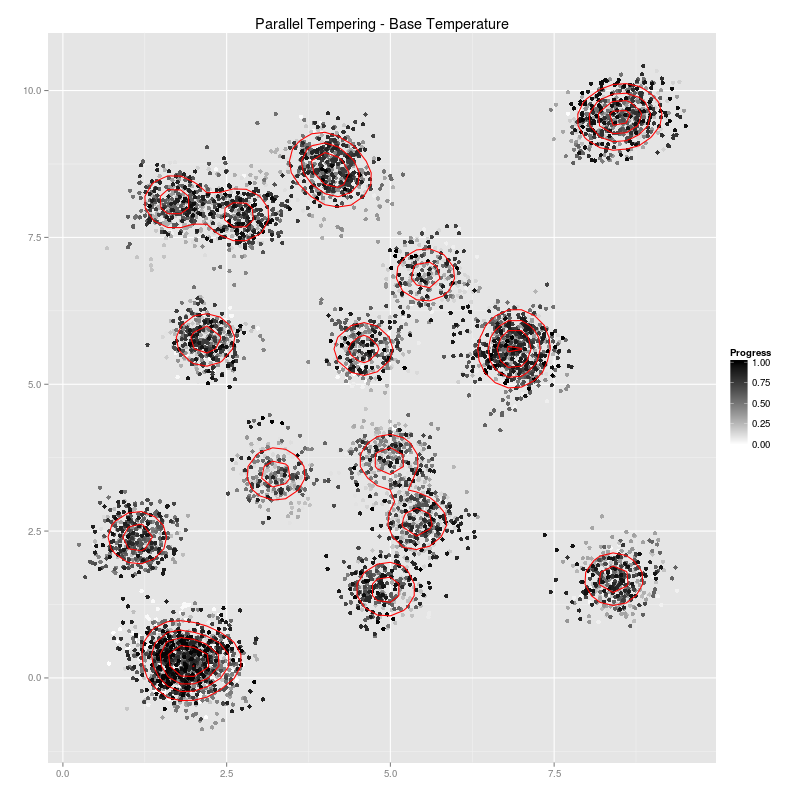
\includegraphics[width=\textwidth,keepaspectratio]{./img/PT_simululation_base_temperature_10000_steps_1.png}
	\caption{Ten Thousand Iterations - about a quarter of which resulted in different points.}\label{PTlong}
\end{figure}	
	
	\chapter{ Theory }\label{theory}	
		%!TEX root = <parallelTemperingMaster.tex>

In this chapter we shall expose the theoretical details of the \PT. The following solutions are implemented in the prepared software, as described in Chapter \ref{Implementation}. 

\section*{Problem statement}

Let $(\Omega, \mathfrak{F})$ be a measurable space. $\Omega$ --- the \sspace, a subset of a Polish space, and $\mathfrak{F}$ - countably-generated Borel subsets. Finally, denote the unit interval by $\mathcal{I} = [0,1]$. 

\begin{Problem}
	\item{\label{Problem}
		Given a distribution $\Pi: \mathfrak{F} \mapsto \mathcal{I}$
		\begin{Problem}
		 	\item absolutely continuous with respect to some measure on $\Omega$, with a density $\pi$ that we know to evaluate 
		 	\item density $\pi$ known up to its proportionality factor
		 	\item \label{multiModality}density $\pi$ being multimodal
		\end{Problem} 
		draw a sample $\{ X_1, \dots, X_\nn \}$ from $\Pi$ so that for any function $g \in \mathbb{L}^1(\Pi)$ one can approximate well the integrals with empirical means
		$$\int_\Omega g \,\dip \approx \frac{1}{\nn}\sum_{i = 1}^\nn g(X^{[i]}). $$ 
	}
\end{Problem}

The rather abstract setting might seem to be an overshot, because, as the reader suspects, the most obvious and natural choice would be that of $\Omega = \real^\nn$ and $\mathfrak{F}$ the corresponding Borel sets. That, however, is not always the case --- for very often one encounters some discrete spaces as well. Moreover, the abstract setting underlines the modularity of the implementation of the algorithm itself, being described in CHAPTER.

Had it been that $\pi$ was not multimodal then by using the usual Metropolis-Hasting algorithm one could have easily solved the \ref{Problem}. Adding condition \ref{multiModality}, however, makes the use of that algorithm problematic because of its localness --- a phenomenon well visualised in CHAPTER.

%%%%%%%%%%%%%%%%%%%%%%%%%%%%%%%%%%%%%%%%%%%%%%%%%%%%%%%%%%%%%%%%%%%%%%%%%%%%%%%%%%%%%%%%%%%%%%%

\subsection*{The \PT} 
The Parallel Tempering algorithm is based on the idea of extending our attention to the product space $(\Omega^\lll, \mathfrak{F}^{\otimes \lll}, \pi_\beta)$ equiped with a specific Markov chain\footnote{Here $\mathfrak{F}^{\otimes \lll} \equiv \underbrace{\mathfrak{F} \otimes \dots \otimes \mathfrak{F}}_{\text{L times}}$ is the usual product sigma algebra.}. The main idea is that on each copy of $\Omega$ the corresponding chain will encounter a slightly modified version of the density of interest $\pi$. In the usual \PT\, one settles for 

\begin{assumptions}
	\item $\pi_\beta \propto \pi^{\beta_1} \times \dots \times \pi^{\beta_\lll},$\label{product form}
\end{assumptions}	

where $\beta = (\beta_1 , \dots , \beta_\lll)$ are such that $1 = \beta_1 > \dots > \beta_\lll > 0$. Their inversions, $T_i = \frac{1}{\beta_i}$, called temperatures, do form therefore a growing sequence of numbers. This naming convention finds its origin in the use of the \PT\, in Statistical Physics where the $T_i$ parameters had direct interpretation. 

We do stress that the normalising constants for each $\pi^{\beta_l}$ are not assumed to be known, as we might not even know it for $\pi$ itself.

A Markov Chain\footnote{For the algorithm step numbering we shall henceforth use the square brackets notation.} $X \equiv \{ X^{[k]}\}_{k \geq 0}$ is then constructed on $\Omega^L$. Its construction makes explicit use of two kernels that make direct reference to $\pi^\beta_l$ --- first one, being a standard \randomWalk, is responsible for the exploration of the \sspace. The other, called the \swapStep, takes care of communication between different subchains ---  for $X$ can also be thought of as being a collection of coordinate subchains 
$$X^{[k]} = (X_1^{[k]}, \dots, X_\lll^{[k]}).$$
Observe that the first subchain corresponds to the solution of the \ref{Problem}.

The main idea behind the construction of chain $X$ is that the subchains operating on tempered versions of $\pi$ influence the subchains linked with lower temperatures by offering them their own accepted proposals. This should be highly beneficial, as more tempered chains will encounter less problems in accepting proposals from regions where the first chain would hardly ever stray.  

To make this approach work at all we are still bound to make some other assumptions. 

\begin{assumptions}[resume]
	\item The starting points $X^{[0]}$ are selected so that $\pi(X_l^{[0]}) > 0$ for $l \in \{1,\dots,\lll\}$.\label{beginAtFullProbabilitySet}
\end{assumptions}
	
Obviously, what follows is that $\pi(X_l^{[0]})^\beta_k > 0$ as well. It is important, for otherwise, what will be demonstrated in the following sections, the algorithm would be dividing by $0$ and break. Moreover, what follows from \ref{beginAtFullProbabilitySet} is that the algorithm will never find itself in a point on which the density evaluates to zero.  

The choice of modifying $\pi$ by exponentiation, as in \ref{product form}, besides its simplicity\footnote{For in general one could settle for some other kind of homotopic deformation.}, has considerable advantages in the analysis of the algorithm. For in the \randomWalk\,phase of the algorithm's step suppose a proposal $y$ is generated by the $l^\text{th}$ chain from a region with less $\Pi$ probability on it in comparison to the position $x$ occupied in the last step, so that $\pi(y) < \pi(x)$. What follows,

$$ 
	\alpha_{\beta_l}(x,y) =  1 \wedge \Biggl(\frac{\pi(y)}{\pi(x)}\Biggl)^{\beta_l} = 
	\Biggl(\frac{\pi(y)}{\pi(x)}\Biggl)^{\beta_l} > \frac{\pi(y)}{\pi(x)} = 1 \wedge \frac{\pi(y)}{\pi(x)} = \alpha_{\beta_1}(x,y),
$$

which means that the probability of accepting such a proposal is larger on the more tempered chains. On the other hand, if  $\pi(y) > \pi(x)$, then this probability remains the same, $\alpha_{\beta_1}(x,y) = \alpha_{\beta_k}(x,y)$. This assures that more tempered chains can make longer excursions into regions not so much $\Pi$-probable. 

One cannot neglect one possibility though: if the support of $\pi$ is not connected and the connected components are far away then it is highly improbable that the algorithm will give unbiased results because of poor mixing that cannot be fixed by exponentiation and some other technique should be used. We stress this point because in computer simulations one might tumble upon this problem because of the finite arithmetic --- the rounding of numbers to zero.    

As pointed out before, the update mechanism of the \PT\,consists of two stages. Assume that the algorithm has reached $n^\text{th}$ step, $X^{[n-1]}$. Following notation used in \citet*{BM1}, we introduce two kernels that act subsequently on $X^{[n-1]}$

$$X^{[n-1]} \overset{\metro}{\rightarrow} \widetilde{X}^{[n-1]} \overset{\swap}{\rightarrow} X^{[n]}.$$

We shall refer to $\swap$ and $\metro$ as to the swap kernel and the random-walk kernel respectively\footnote{$M$ as Metropolis.}. These will be now presented in greater detail.



	\subsubsection*{The \randomWalk\, Kernel}
	
Take a point in the \sspace, $x = (x_1, \dots, x_\lll) \in \Omega^L$. To assign probabilities to the proposal of the next step, given $x$, we consider events $A_i \in \mathfrak{F}$. We shall assume that 

\begin{assumptions}[resume]
	\item{
		\randomWalk\, proposal generation occurs independently on all subchains 	
		$$\metro (x, A_1 \times \dots \times A_L) = \prod_{l=1}^L \metrobis{l}(x_l, A_l).$$
	}
\end{assumptions}

The $\metrobis{l}(x_l, A_l)$ corresponds to standard Metropolis kernel, as in \citet*{CharlesJ.Geyer}. To be more precise

\begin{equation}\label{metropolisKernel}
	\metrobis{l}(x_l, A_l) \equiv \int_A \alpha_{\beta_l} (x_l, y_l) q_{\Sigma_l} (y_l - x_l) \mathrm{d }y_l + \iii(x_l,A) r(x_l) 	
\end{equation}

where 
$$r(x_l) = \int [1 - \alpha_{\beta_l} (x_l, y_l)] q_{\Sigma_l} (y_l - x_l) \mathrm{d }y_l$$
is the probability of not accepting the proposal and the subprobability density of accepting the update \footnote{Also known as the Hastings ratio.} is

\begin{equation}\label{acceptance prob}
	\alpha_{\beta_l} (x_l, y_l)  \equiv 1 \wedge \frac{\pi^{\beta_l}(y_l)}{\pi^{\beta_l}(x_l)}.
\end{equation}

To understand why $\metrobis{l}$ is given by Eq. \ref{metropolisKernel} we note that the role of the kernel is to assign probability to the next step of the algorithm given that the previous one assumed value $x$\footnote{So we abstract here from how the actual value $x$ was obtained, being mysteriously revailed to us by Nature, under the guise of random number generator. In fact kernels and their duals play principal role in the Bayesian statistics.}. The \MH\, goes as follows\footnote{We omit the inverse temperatures for time being.}: 

\begin{Algo}[Metropolis-Hastings]
	\ 	
	\begin{algorithmic}
		\Require $X^{[0]}$ such that $\pi(X^{[0]}) \not=0$
		\Procedure{\textsc{Metro}}{$X^{[0]}$, $N$}
			\For{$n \in \{0, \dots, N-1\}$}
				\State Draw proposal $Y \sim q(X^{[n]},y)\mathrm{d}\,y$
				\State Draw $U \sim \mathcal{U}(0,1)$
				\If{$U \leq \alpha(X^{[n]},Y)$}
					\State $X^{[n+1]} \gets Y$	
				\Else
					\State $X^{[n+1]} \gets X^{[n]}$	
				\EndIf
			\EndFor			
		\EndProcedure	 
	\end{algorithmic}		
\end{Algo}

Therefore, one should assign probability to event $\{ X^{[n+1]} \in A\}$ for all $A \in \mathfrak{F}$. But this is done, as

$$\int_A  \alpha(x,y) q(x,y) \mathrm{d}\,y = \int_A \prob \Big( U \leq \alpha(x,y) \Big)q(x,y) \mathrm{d}\,y =$$
$$
	=\int_A \prob\Big( U \leq \alpha(x,Y) | Y=y \Big)q(x,y) \mathrm{d}\,y = \prob\Big( U \leq \alpha(x,Y), Y \in A \Big)=
$$
$$
	= \prob\Big(X^{[n+1]} \not= X^{[n]} , X^{[n+1]} \in A \Big)
$$

where we assume $Y$ to be drawn out of the proposal distribution and $U$ to be independent of it. Setting $A = \Omega$ one notices that\footnote{Under the sensible assumption that the proposal distribution does not have any atom in $x$ --- this is usually automatically assumed by considering a distribution that is absolutely continous w.r. to Lebesgue measure.} 

$$ \prob\Big(X^{[n+1]} = X^{[n]}\Big) = \int  [ 1 - \alpha(x,y)] q(x,y) \mathrm{d}\,y = r(x)$$
--- precisely as claimed. 

In the above equations the proposal distribution being used, following notation from \cite{CharlesJ.Geyer}, is $q(x_l,y_l) = q_{\Sigma_l} (y_l - x_l)$, where $q_{\Sigma_l}$ is the density of $\mathcal{N}(0, \Sigma_l)$. 

The simple form of Eq. \ref{acceptance prob} stems from proposal distribution symmetry, $$q(x_l,y_l) = q(y_l,x_l).$$

The choice of $\alpha$ is motivated by assuring the self-adjointness of the $\metro$ operator, which in turn implies that distribution $\Pi$ is preserved, so that
	
\begin{equation}
	\Pi \metro = \Pi.		
\end{equation}	

As indicated by \cite{BM2}, the implementation of $\metro$ consists of separate simulation of $\metrobis{l}$ for each of the coordinate chains,  $X^{[n-1]}_l$.

	\subsection*{The swap kernels}

Now we address the question of how to interlace the independent chains generated with kernel $\metro$. We want to swap the generated states so that chains with higher temperature influence the regions of lower temperatures. Being more precise, the swapping gives some possibility to the chains with lower temperatures to find themeselves in states that would otherwise be very unlikely to happen, the path leading to them being very unlikely to occur - these paths are rendered more probable for the chains with higher temperature. The swaps are made at random so that the probability of swaps takes into account some properties of $\pi$ evaluated on the last points from all the chains. 

Before passing to detailed description of different ways the swaps might be made, which we call \strats, let us first describe the properties of the swap kernel $\swap$ common to all \strats. In all cases, we rely on the following assumption

\begin{assumptions}[resume]
	\item At one step of the algorithm, there will be only one possible swap between a chosen at random pair of coordinates.
\end{assumptions}

The restriction here is not so much in the number of swaps per step. What seems to be more relevant is rather the constraint to a particular subset of the group of all permutations --- for one could certainly envisage that any random permutation could take place. However, it simplifies the interpretation of \strats\, that are to be described. 

Let us denote the swap operator by $S_{ij}$, so that 
$$S_{ij} x = (x_1, \dots, x_{i-1}, x_j, x_{i+1}, \dots, x_{j-1}, x_i, x_{j+1}, \dots, x_L).$$ 
We require $\swap(x, \circ )$ to be a measure concentrated on the set of all possible pairs of swaps between coordinates of $x = (x_1, \dots, x_L)$, i.e. on the set $\mathfrak{S}_x \equiv \{ S_{ij}x : i < j  \}$. We note that the proposal measure for the swap kernel $\mathcal{Q}$ is of the following form 

\begin{equation*}
	\mathcal{Q}(x, A) \equiv \underset{i < j}{\sum} p_{ij}(x) \mathbb{I}_A (S_{ij} x)
\end{equation*}	 

Then, the swap kernel would be of the following form, for any $x \in \Omega^L$ and $A$

\begin{equation*}
	\swap(x,A) = \int_{A} \alpha_\text{swap} (x,y) \mathcal{Q}(x, \mathrm{d}\,y) + r(x) \mathcal{I}(x,A)
\end{equation*}	

where $r(x) = 1 - \underset{\Omega^L}{\int} \alpha_\text{swap} (x,y) \mathcal{Q}(x, \mathrm{d}\,y) $. Plugging $\mathcal{Q}$ permits us to write

\begin{align*}
	\begin{split}
		\int_{A} \alpha_\text{swap} (x,y) \mathcal{Q}(x, \mathrm{d}\,y) &= \underset{ i < j}{\sum} p_{ij}(x) \int \alpha_\text{swap} (x,y) \mathbb{I}_A (y) \delta_{S_{ij}x}(\mathrm{d}\, y) \\ &= \underset{ i < j}{\sum} p_{ij}(x) \alpha_\text{swap} (x, S_{ij}x) \mathbb{I}_A(S_{ij} x),
	\end{split}
\end{align*}	

so that finally

\begin{equation*}
	\swap(x,A) = \underset{ i < j}{\sum} p_{ij}(x) \alpha_\text{swap} (x, S_{ij}x) \mathbb{I}_A(S_{ij} x) + \Big( 1 - \underset{ i < j}{\sum} p_{ij}(x) \alpha_\text{swap} (x, S_{ij}x)\Big) \mathcal{I}(x,A),
\end{equation*}	

where 

	$$\alpha_\text{swap}(x,y) = \frac{\pi_\beta( \mathrm{d}\, y ) \mathcal{Q}(y, \mathrm{d}\,x)}{\pi_\beta( \mathrm{d}\, x ) \mathcal{Q}(x, \mathrm{d}\,y)} \wedge 1$$

is the Radon-Nikodym derivative of two measures. It's calculated with respect to measure $ \mu (\mathrm{d}\,x, \mathrm{d}\,y) \equiv \pi(\mathrm{d}\,x) \mathcal{Q}(x, \mathrm{d}\,y)$. The measure that is being differentiated is $\mu$ composed with the exchange coordinates operation, $R(x,y) = (y,x)$\footnote{Which is obviously measurable in the appropriate sense.}. So finally $\alpha_\text{swap} \equiv \frac{\mathrm{d}\, \mu \circ R^{-1}}{\mathrm{d}\, \mu}$.

Observe that thanks to the proposal's support finiteness we actually get 

	$$\alpha_\text{swap}(x,y) =  \frac{\pi_\beta( y ) \mathcal{Q}(y, x)}{\pi_\beta( x ) \mathcal{Q}(x, y)} \wedge 1.$$


Now, since $y \in \mathfrak{S}_x $, the tagetted $\pi_\beta$ is a tensor of measures, $Q(x, S_{ij} x) = p_{ij}(x)$, and $Q( S_{ij} x, x) = p_{ij}(S_{ij}x)$ \footnote{Here we pass from measure notation to probability function notation, $\mathcal{Q}(x, \{S_{ij}x \}) = \mathcal{Q}(x, S_{ij}x)$. We can do it because $\mathcal{Q}$ is purely atomic given $x$.}, we get finally 

\begin{equation*}
	\alpha_\text{swap}(x,S_{ij} x) = \Big[  \Big(\frac{\pi(x_j)}{\pi(x_i)} \Big)^{\beta_i - \beta_j}  \frac{ p_{ij}(S_{ij} x )}{ p_{ij}( x ) }\Big] \wedge 1
\end{equation*}	

In our computer simulations several swapping strategies have been tested. For instance,

\begin{strategy}
	\item 
		$
			p_{ij}(x) \propto 
			\frac{\pi (x_j)}{\pi( x_i )} \wedge \frac{\pi (x_i)}{\pi( x_j )} = 
			\exp \Big( - \big| \log ( \pi(x_j) ) - \log ( \pi(x_i) ) \big| \Big).
		$\label{strat1} 
\end{strategy}

In this particular the proportionality is in fact equality, because the above expression is transposition symmetric and this considerably simplifies the statistical sum analysis. In general, we want $p_{ij}(x) \propto h(x_i,x_j)$ for some function $h$. Thus,

\begin{equation*}
	\frac{p_{kl}(S_{kl}x)}{p_{kl}(x)} = \frac{\frac{h(x_l,x_k)}{A(\tilde{x}_{kl})+f(x_k)+g(x_l)+h(x_l,x_k)}}{
	\frac{h(x_k,x_l)}{A(\tilde{x}_{kl})+f(x_l)+g(x_k)+h(x_k,x_l)}
	} = 
	\underbrace{\frac{h(x_l,x_k)}{h(x_k,x_l)}}_\text{'direct effect'} 
	\times 
	\underbrace{\frac{A(\tilde{x}_{kl})+f(x_l)+g(x_k)+h(x_k,x_l)}{A(\tilde{x}_{kl})+f(x_k)+g(x_l)+h(x_l,x_k)}}_\text{'distribution effect'},	 	 	
\end{equation*}  
where $\tilde{x}_{kl}$ is $x$ without its $k^\text{th}$ and $l^\text{th}$ coordinates, $f(x_l) = \sum_{i<l, i\not=k} h(x_i, x_l)$, and $g(x_k) = \sum_{j>k, i\not=l}h(x_k, x_j)$. As we see it is fairly straightforward to compare the above expression to $1$ if the 'distribution effect' equals $1$, and difficult had it been the other case. To assure this happens, one can settle for a function $h$ that is transposition invariant, $h(x,y)=h(y,x)$. This is certainly the case of \ref{strat1}. In this strategy therefore we are promoting exactly swaps between coordinates whose proposals have relatively the same $\pi$ density values, i.e. $\pi (x_j) \approx \pi (x_i)$. 



\begin{strategy}[resume]
	\item 
		$
			p_{ij}(x) \propto 
			\frac{\pi (x_j)}{\pi (x_i)} \wedge 1 = 
			\exp \Big( - \big[ \log ( \pi(x_j) ) - \log ( \pi(x_j) ) \big]\Big) \wedge 1.$\label{strat2}
\end{strategy}

This strategy breaks the symmetry of the previous one rendering the evaluation of the effect on the $\alpha_\text{swap}$ challenging, if not impossible. The main idea behind this strategy was to  


The subsequent strategies are again functions of the fist strategy.

\begin{strategy}[resume]
	\item 
		$p_{ij}(x) \propto 
			\Big( \frac{\pi (x_j)}{\pi( x_i )} \wedge 
			\frac{\pi (	x_i)}{\pi( x_j )} \Big)^{|\beta_i - \beta_j|} = 
		\exp \Big( - |\beta_i - \beta_j| \times \big| \log ( \pi(x_j) ) - \log ( \pi(x_i) ) \big| \Big).$\label{strat3} 
\end{strategy}

This strategy permits us to soften a bit the requirement that $\pi(x_j) \approx \pi (x_i)$. This effect is strengthened for coordinates that are similarly tempered, i.e. where $\beta_i - \beta_j \approx 0$. Swaps between adjacent chains will be therefore more probable. 

One can also use a strategy that incorporates some distance measure between points, $\rho$ being any quasi-metric. \ref{strat4} is a good example of such procedure - the more distant the points, the less probable it is for them to get swapped.  

\begin{strategy}[resume]
	\item 
		$p_{ij}(x) \propto \Big( \frac{\pi (x_j)}{\pi( x_i )} \wedge \frac{\pi (x_i)}{\pi( x_j )} \Big)^\frac{|\beta_i - \beta_j|}{1 + \rho(x_i, x_j)} = \exp \Big( - \frac{|\beta_i - \beta_j| \times | \log ( \pi(x_j) ) - \log ( \pi(x_i) ) |}{{1 + \rho(x_i, x_j)}} \Big).$\label{strat4}
\end{strategy} 

Finally, for purposes of comparisons with \citet{BaragattiParallelTemperingWithEquiEnergyMoves}, we include also strategies that are \sspace\, independent, i.e. the probability of swaps does not depend on the evaluations of the density $\pi$ in the sample points. Such na\"ive strategies include 

\begin{strategy}[resume]
	\item $p_{ij} = \frac{2}{\lll (\lll - 1)}$\label{strat5}
\end{strategy}

and 

\begin{strategy}[resume]
	\item $p_{ij} = \frac{1}{\lll - 1} \ind{\{|i-j|=1\}}$\label{strat6}
\end{strategy}

amounting to choosing uniformly among all possible swaps and all neighbouring-in-temperature swap respectively. 
	
	
The implementation of the template was carried out using the \RR\, programming language. The intention behind this choice is its popularity among users that are not necessarily computer scientist, but practitioners using statistical simulations on the day-to-day basis. 
\chapter{ Implementation }\label{Implementation}

In this chapter we will present the implementation of the \PT. 

The analysis of the algorithm in all its complexity called for the development
of a more structurised template for carrying out numerical computations. The
\PT, being an extension to the \MH, would naturally share many similarities in
implementation when compared to the \PT. Both algorithms can have very
abstract formulations and can be carried out theoretically on any countably-
generated measurable space. Practical considerations will never go that far.
However, one cannot, in principle, discard the use of Stochastic Simulations in solving many real-life modelling problems, i.e. Bayesian model selection, or in doing calculations on lattices when considering the 
Ising model of crystallic structures. The mulitude of potential applications call for potentially flexible implemention of the \PT\, was a flexible one. To attain this goal, the object-oriented paradigm was applied, so that the \sspace\, and the \algo\, were conceived as two separate entities, as a possible
solution to the upper-mentioned problem.

Having realised the need for modularity, it seemed natural to take the whole idea one step further and develop a general template for Metropolis-Hastings-like simulations, going way beyond the idea of a task-specific computer programme. For there are other potential developments of the \MH\, that are being used. There are many similarities in stuctures of these algorithms. Our template's goal was therefore to provide basic building blocks used for simulations, leaving the practitioners concentrate on the analysis. To guarantee user-friendliness, the most common State Space, the multidimensional euclidean space, has been provided, so that the user could in principle carry out computations specifying only the required minimum - the density function of the measure of interest. With future releases of the software, more standard State Spaces are scheduled for implemention as well, giving the practitioners experience the potentials and drawbacks of Metropolis-Hastings-like stochastic simulations.

\RR\, offers several implemented meta-structures that enable basic object oriented programming techniques. Among these there are the \textbf{S3} classes, \textbf{S4} classes, and the most recent Reference Classes. The implementation of \Metro\, was carried out using Reference Classes. This choice was dictated by several reasons. First, only \textbf{S4} classes and Reference classes offer the possibility of basic type verification\footnote{Still far from the \Cpp\, standards though.}. This assured that no serious errors were introduced in the implementation phase and that users cannot provide absurd input for the algorithm. Moreover, the Reference Classes are the only implementation of objects that use passing arguments by reference, that a priori could saved some time in the calculations on unnecessary object copying\footnote{Altough no serious differences in execution time were actually spoted when comparing both the functionally programmed prototype with the object-oriented final version.}. Finally, the Reference Classes are considered to be highly compatible with \Cpp\, precompiled programmes called from \RR. This is a clear advantage, as the future shipments of \Metro\, are planned to be implemented in \Cpp, so that users can simulate faster that the whole programme was more memory efficient.   
		\section{Division into objects}

To assure real modularity of our template, more divisions were proposed than only the one mentioned at the beginning of this chapter; their structure being represented in Figure \ref{objectStructure}.

We already mentioned the separation of the Algorithm from the State Space. It is useful to think of the Algorithm as of a decision-maker. Its role is restricted to making decisions on acceptance or rejections of the proposals generated by the State Space and then on ordering the State Space to perform all the subsequent actions. The information on which the Algorithm bases its decisions depends on the points from the State Space only indirectly, via the evaluations of densities ( or, in the discrete case -- probability functions ) at the proposal points. A third candidate for an entity thus appears - namely an object whose methods would serve to measure some characteristic of the State Space sample points for the use in the decision-making of the Algorithm. We called this entity the Target Measure. 

The very idea behind the Target Measure entity is that it should serve as a container for user-defined probability function or a density together with every additional data-structure required for its evaluation. Moreover, in case the user was interested in testing the \PT's potential on some toy-example, that was analytically tractable or could be simulated using any other simpler and more efficient technique, the Target Measure entity would be the place to store any additional methods tied with this particular distribution. For example, in our simulations (confront Chapter \ref{simulationsAndResults}) we could  additionally provide efficient methods for quantile simulations and evaluates of the real distribuant. Implementations of these functions were collected as methods of the appropriately named instatiation of the Target Measure structure.  

\begin{figure}
	\centering 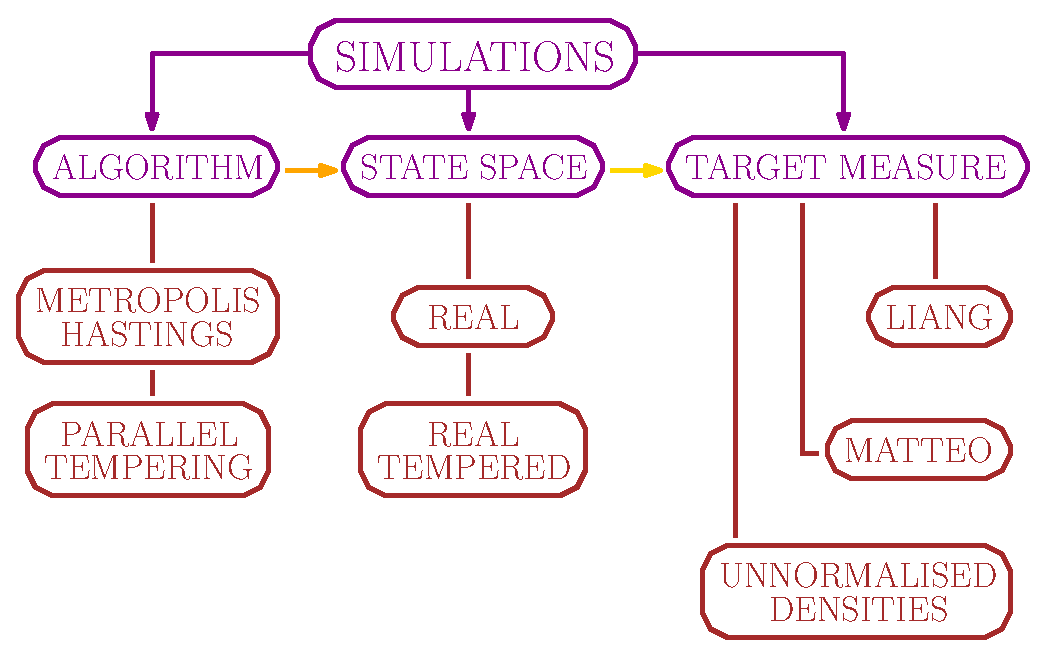
\includegraphics[keepaspectratio=true, width =\linewidth]{./img/objectStructure.eps}
	\caption{Current operational entity-relations diagram.}\label{objectStructure}
\end{figure}

The reason for separating the Target Measure from the State Space is again dictated by the modularity requirement. Totally different models can be modelled on the same State Space, the only difference being the way the probability is assigned. It is therefore natural to define an entity whose task will be to serve as a warehouse for sample points, together with efficient methods or reading them, and in the end -- presenting the results to the user. These things, to some extent, can be done for any probability measure defined by the user. 

The Object Oriented paradigm gives the programmer the tool of inheritance. Its role is to assure no code copying when several programmes share the same structure and differ only at some minor implementation details. In this implementation we have noticed that the \PT, being an extension to the \MH, differs only in the appearance of the swap stage and its methods, the Random Walk stage being almost the same\footnote{The difference being that it is called for several chains instead of one.}.    

All the entities must be linked, so that different parts of programme could call methods of other entities. Because of certain Reference Classes limititions\footnote{As pointed out before, Reference Classes are relatively new, and, as such, poorly documented. With trial and error it has been checked, that this particular choice of entity-nesting simply works.}, the Algrorithm has a pointer on the State Space, which in its turn has a pointer on the Target Measure. These relationships are visualised in Figure \ref{objectStructure} under the form of golden arrows. Under different circumstances, different realisations of objects will appear as the Algorithm, the State Space, and the Target Measure. For instantance, if the user wanted to carry out standard Metropolis-Hastings calculations on the three-dimensional euclidean space and check how it copes with the density function he provided, then the programme would have to initialise first the Unnormalised Density as the realisation of the Target Measure entity. Then, initialise the Real space as an instatiation of the State Space and set the pointer for the previously initialised. Finally, it would initialise the Metropolis-Hastings as the operational Algorithm and set the pointer on the previously initialised State Space, being the Real space. To automate this chain of initialisations, a controller entity was established under the name of Simulation ( see Figure \ref{objectStructure} ). Two additional functions were written, \textsc{Metro} and \textsc{PT}, serving as wrappers to the more general Reference Class constructor of the Simulation object. 

Continuing on the example, the user would simply had to call

\begin{lstlisting}
	Example <- Metro(
		n = 1000,
		space = 'real',
		spaceDim = 2,
		targetDensity = userDefinedDensity
	)
\end{lstlisting}  
where \textsc{userDefinedDensity} is an R-implemented unnormalised density function\footnote{In future versions \Cpp\, calls will be usable.}.  

The presented object structure is far from final. Hopefully it will evolve in time, trying to match the needs of various users. We already plan the separation of the swap distributions from the Parallel Tempering entity, giving the user the possibility to check his own swapping strategies, possibly better suited for their needs.
		\section{Functions and Methods}

Here we shall give a brief description of the functions callable after the loading of \Metro\, Package.	
		\section{Two-dimensional Колмогоров-Смирнов distance}

In order to check how different strategies approximate the toy-example distribution described in the next chapter, one had to settle for some kind of criterion. Because the general task is to approximate the integral 

$$ \expect f( X ) \text{  ,  } X \sim \pi$$

it is natural to settle for the Колмогоров-Смирнов distance, given by 

\begin{equation}\label{KS definition}
	\underset{x \in \real^\kk}{\sup} | F(x) - \hat{F}_\nn (x)|,
\end{equation}

where \Fecdf\, is the Empirical Cumulative Distribution Function, \ecdf , constructed from the chain generated by the \PT. 



The naturality of our criterion stems from the simple observation, that in practice we often forget that the whole \ecdf\, generated this way is a random measure, being extracted from a trajectory of the underlying stochastic process, and use it as a proxy for the real measure $\pi$. And so it seems natural to check for the distance expressed in equation \ref{KS definition}. 

ADD HERE THE VITALI SPACE

Suppose we are given a simulation with $\tilde{\nn}$ iterations after the burn-in period. It often happens that the algorithm stays for more than one iteration in certain sample points\footnote{In fact we can easily control the point sejour-time due to the random walk by manipulating the proposal step's distribution parameters. In case of the kernel generated by the conditional normal distribution, it suffices to diminish the entries of the covariance matrix.}. We count the occurences of that points and then normalise them dividing them by $\tilde{\nn}$ and call the result {\it a charge}. Thus, we are given a matrix with sample coordinates and their charges. If the target measure $\pi$ is absolutely continous with respect to the Lebesgue measure, then the points generated by accepted proposals should all differ on both of their coordinates, the measure of any submanifold of $\real^\kk$ being zero. If that is not the case, then we simply face the problem of computer's finite arithmetics and could solve it by a longer binary representation of the real numbers. In practice that is an extremely unlikely event and we will neglect it. Therefore we will from now on focus on points with distinct coordinates and refer to the number of thereof by $\nn$. The world {\it sample} will also be applied only to the uppermentioned points. 

The computations of the \KS might be computationally expensive, requiring, in pesimistic case, evaluation of the true Cumulative Distribution Function $F$ in approximately $\frac{\nn^\kk}{\kk!}$ points\footnote{The exact number being equal to number of points on the intersection of a $\kk+1$ dimensional simplex with the coordinates summing to $\nn$, and the $\mathbb{Z}^{\kk+1}$ lattice.}. To see that, let us focus in all of this section on the bivariate case\footnote{\dots the generalisation to higher dimension being straighforward.}.   


\begin{figure}
	\centering 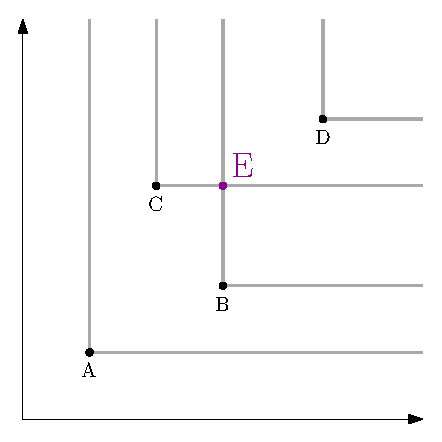
\includegraphics[scale=1]{./img/KS1.eps}
	\caption{Sample points and level sets of an examplary \ecdf.}\label{simpleEcdf}
\end{figure}


Observe, that the level sets of any \ecdf\, are uniquely determined by the sample points ( as $A, B, C$ and $D$ in Figure \ref{simpleEcdf} ) and points generated from them by taking the vectorised maximum

$$ 
	\begin{bmatrix} a_1 \cr a_2 \end{bmatrix} \vee 
	\begin{bmatrix} b_1 \cr b_2 \end{bmatrix} = 
	\begin{bmatrix} a_1 \vee b_1 \cr a_2 \vee b_2 \end{bmatrix},
$$ 
( such as $E$ in Figure \ref{simpleEcdf} ).  

One of the easiest way of establishing the values on the level sets of \Fecdf  is by considering a square, $(\nn+2)\times(\nn+2)$ matrix $B$, as in Figure \ref{spaceDivision}. The entries of $B$ correspond to values of \Fecdf\, on certain rectangles. Take the set of all $x$-coordinates of sample-points, $\Phi_x$, and the set of all $y$-coordinates of sample-points, $\Phi_y$. Add to them the coordinates of two dummy points: $(x_0, y_0)$ and $(x_{\nn+1}, y_{\nn+1})$ We enumerate points of these sets in the ascending order, $\Phi_x = \{ x_0 < x_1 < \dots <x_\nn < x_{\nn+1} \}$ and $\Phi_y = \{ y_0 < y_1 < \dots <y_\nn < y_{\nn+1} \}$. Then, the \Fecdf\, function is constant on rectangles 

$$R_{ij} = [x_i, x_{i+1})\times[y_j, y_{j+1}),$$ 
where $i,j \in \{0, 1, \dots, \nn+1 \}$. It is easy to realise now, that the number of level sets depends on the number of sample points and points generated by them using the vectorised maximum, $\hat{\nn} = \# \{ z : \exists x,y \in \text{Sample} x,y \not=z \text{ and } z = x \vee y \}$. This number is easily seen to be the greatest if all sample points could be arranged so that their $x$-coordinates strictly increase and $y$-coordinates strictly decrease.  

To actually derive the \KS\, we must assume that we can evaluate not only the true \cdf\, $F$, but also its two marginals\footnote{Limits of all the possible subsets of coordinates in infinity.}. Similarly to its univariate counterpart, the \KS\, can be calculated on only a finite number of points. Consider any rectangle. \Fecdf\, is constant on it. So the \KS depends solely on the evaluations of $F$ on that set. But $F$ is a distribuant - a function monotone in all its arguments, and so the maximum distance from \Fecdf\, can be attained only on the vertices of the rectangle. On the border rectangles ( $R_{i,\nn+1}$ and $R_{\nn+1,j}$ ) the evaluation simplifies to vertices adjacent to $R_{ij}$ rectangles and it is there, where we have to evaluate the marginals instead of $F$. \Fecdf\, is equal to zero on rectangles on the southern and western extremities. Thus we put $B_{i0} = B_{0j} = 0$. 

\begin{figure}
	\centering 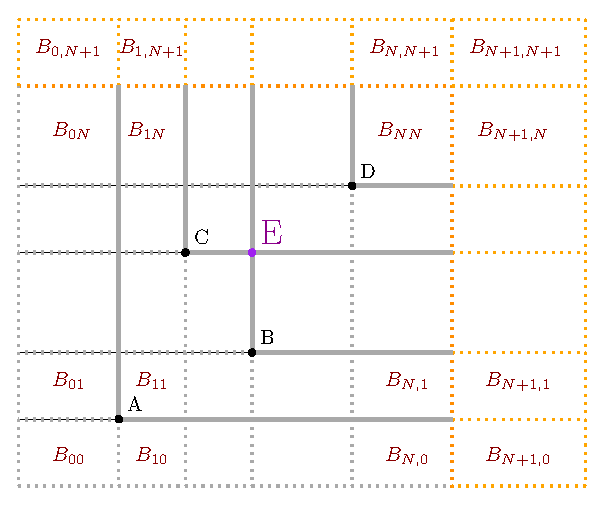
\includegraphics[scale=1]{./img/KS2.eps}
	\caption{Sample points and level sets of an examplary \ecdf.}\label{spaceDivision}
\end{figure}


The rest of the algorithm is based on the dynamic programming approach introduced by \citet*{NiVingron} for comparing lists of changes in gene expression under different scoring regimes. The overall algorithm proceeds as follows:

\begin{minipage}[h]{\linewidth}
\begin{algorithm}
	\item Let $KS := 0$, $\jj = \nn+1$. 
	\item Read $\alpha$
	\item Prepare $\Phi_x$ and $\Phi_y$.
	\item While $i \in \{1, \dots, \nn+1\}$, and while $j \in \{ 1, \dots, \ii \}$ 
	\begin{algorithm}
		\item $B_{ij} := 
			\begin{cases} 
				B_{i-1,j-1} + \text{adequate charge}, \text{ if $R_{ij}$'s upper-left vertex is a sample-point} \cr
				B_{i,j-1} + B_{i-1,j} -  B_{i-1,j-1}, \text{ Otherwise} 
			\end{cases}$	

		\item\label{whenToEvaluate} If $i,j < \nn+1$ and both $B_{ij} > B_{i,j-1} \vee B_{i-1,j}$, then evaluate $F_{ij} = F(x_i, y_j)$.

		\item If either $i$ or $j$ equals $\nn+1$ evaluate the marginal distribtion.

		\item\label{changes} Evaluate $|F_{ij} - B_{ab}|$ at $a \in \{i-1,i\}$ and $b \in \{j-1,j\}$ or only on $i-1$ and $j-1$ if on border. If it is bigger than $KS$ then update $KS$. If the update occured and the new $KS$ is such, that $F_{ij}\wedge B_{ij} > 1 - KS - \alpha$ then update $\jj$ to $j-1$.

		\item Increase $j$ by one. After the end of loop increase $i$ by one.

	\end{algorithm}
	\item Return $KS$.
\end{algorithm}
\end{minipage}



Important changes with respect to \cite{NiVingron} can be seen in point \ref{changes} and the introduction of two extra variables $\jj$ and $\alpha$. The introduction of $\jj$ stems from the easy observation, that if both distribuant $F$ and \Fecdf\, are already in the interval $(1-KS,1]$, then any further evaluations of $KS$ to the East and North could not result in a bigger difference then the one already observed. Parameter $\alpha$ gives a further reduction in the number of calculations, enlarging that band to $(1-KS-\alpha,1]$, so that the true \KS will not be larger than by $\alpha$ from the value already established. We have also noted that it is not important to evaluate the real distribuant at every point of the matrix $B$. Rather than that, we note that because $F$ is a distribuant, evaluations are required on South-Eastern edges of the level sets, such as points $A, B, C, D$, and $E$ on Figure \ref{spaceDivision}. That is the reason behind point \ref{whenToEvaluate}. Other changes seem to be of minor importance and result from discretisation of the {\it a priori} continous problem. 


Our impelementation of the \KS calculator might not the optimal one. As pointed out by \citet*{Jon} the problem of calculating values of an \ecdf\, only in the sample points could be solved in $\mathcal{O}(\nn \log( \nn ))$ iterations. The existence of an algorithm requiring only $\mathcal{O}(\hat{\nn} \log( \hat{\nn}  ))$ operations, interesting in its own sake, will be object of further research.

	\chapter{ Simulations and Results }\label{simulationsAndResults}

Recall that Liang-Wang example of a multimodial function:

\begin{equation}\label{againLiang}
f(x) = 
\sum_{i=1}^{20} \frac{\omega_i}{ \sigma_i \sqrt{2 \pi} } \exp \Big( -\frac{(x - \mu_i)^\tran (x - \mu_i)}{2 \sigma_i^2} \Big),	
\end{equation}
where $\sigma_1 = \dots = \sigma_{20} = 0.1$, $\omega_1 = \dots = \omega_{20} = 0.05 $ and the means $\mu_i$ are enlisted in Chapter \ref{motivation}.

Since we are dealing with stochastic simulations, do focus on the first two empirical moments analysis of different statistics in order to get some understanding of which \textsc{Swap Strategies} is better. 
Because of theoretical reasons mentioned in the Chapter \ref{theory}, one might be tempted to compare different \textsc{Swap Strategies} by considering the behaviour of their Колмогоров-Смирнов distance with the true underlying distribution, given by Eq. \ref{againLiang}. To this end the implemented KS statistics calculator was used, see Chapter \ref{KSimplementation}. The overall results are gathered in Figure \ref{KSdistancePlot}. 

The simulations involving the calculation of the \text{KS} statistics were carried out using the same parameters. The chains proposals have had their covariances matrix chosen so that about one in four proposal got accepted, which is the working rule-of-thumb among the practitioners of the stochastic simulation after the seminal work of \cite{ Roberts2001}. The covariances were chosen to be a slightly modified versions of those proposed by \cite{BaragattiLikelihoodFreeParallelTempering}.  Baragatti chosen the matrices to be of the form $T_i^2 \iii$, where $\iii$ is simply a 2 by 2 identity matrix and $T_i$ the $i^\text{th}$ temperature. The modification consisted in premultiplying the frist three matrices by $0.05$ and the last ones by $0.01$. The temperatures were also taken from baragatti and were equal to $T = (\,1,\, 2.8,\, 7.7,\, 21.6,\, 60\,)$. The computation involved 10000 iterations, a fourth of which was neglected being the burn-in period. The initial states were chosen from a uniform distribution on a square $[0,10]^2$ that contains all the means of the distributions that add up to form the considered mixture.


Figure \ref{KSdistancePlot} summarizes results of two different experiments consisting of different number of simulations --- the first of 40, the latter - of 120. There was no particular reason for choosing this amount of simulations --- the time-cost of the simulations that do calculate the KS statistics is however quite long and so we did not manage to collect information on the same number of simulations. The second group has larger standard deviation --- this can be attributed to differences in number of experiments. However what can be compared is the mean of these distributions. Also the standard deviation can be compared within the two groups. One can see that the differences in mean values of the KS statistics are small, possibly neglectable. However it remains a fact, that first three strategies give results that are on average smaller, so that they are closer to the original distibution in the KS sense. This is to say that generally the state-dependent strategies give better estimates than the state independent one, with the notable exception of the \ref{strat4}. One can also notice that the among the first three state-dependent strategies it is \ref{strat3} that has the lowest variance. Among the state independent stragies it also seems plausible not to draw swaps from a space restricted to only neighbouring ones, leaving it possible to exchange accepted proposals in the \textsc{Random Walk} phase between all the chains.   

\begin{figure}[ht]
	\centering 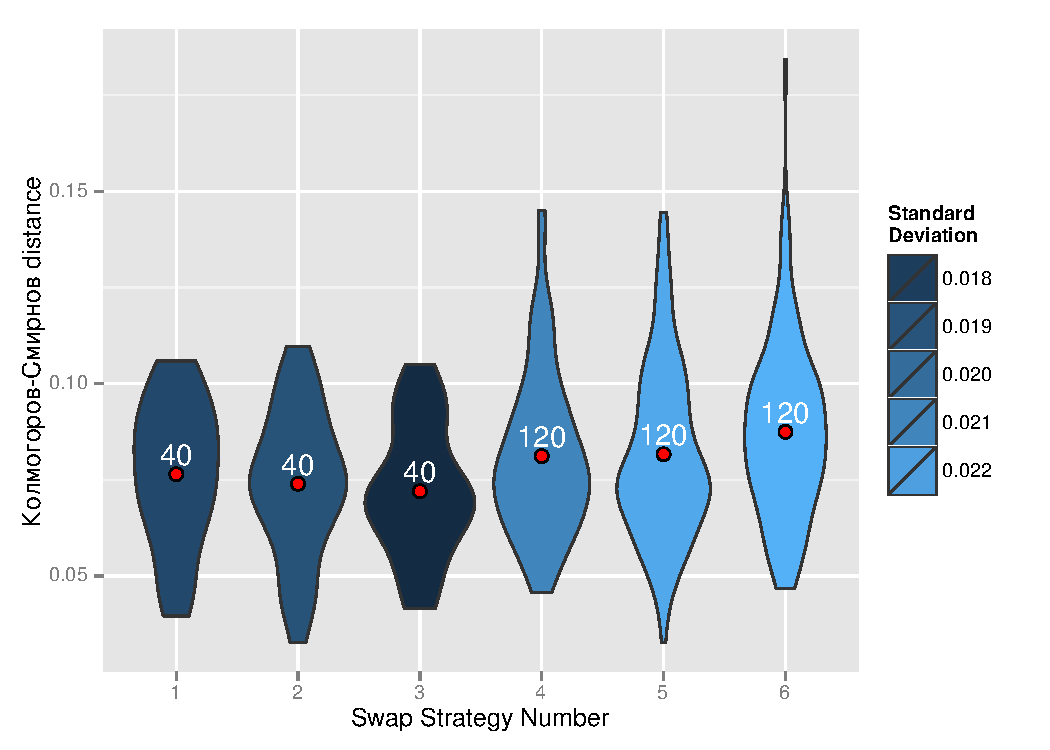
\includegraphics[width=\textwidth,keepaspectratio=TRUE]{./img/KSobs.pdf}
	\caption[Results of the KS-statistics simulations represented by a violin plot.]{Results of the KS-statistics simulations. The number of iterations a particular strategy was tested is annotated with the white numbers just above the red dots. The violin plots are simply smoothened empirical distributions. Red dots are their empirical means. The colour of the violin plots corresponds to the standard deviation, which is more instructive to study when considering subgroups with the same number of simulations.}\label{KSdistancePlot}
\end{figure}


\section{PTEEM as motivation for \textsc{Strategy I}}

One of the aims of the simualation was to compare ourselves with the results of \cite{BaragattiLikelihoodFreeParallelTempering}. In this article the author proposed an algorithm that supposingly combines the good sides of both the \PT\, and the Equi-Energy Sampler, orignally conceived by \cite{ Kuo2006}. The resulting algorithm, called PTEEM, again consists of two steps. In the original article it is assumed that the probability one faces is uniquely defined by a hamiltonian that describes the energy levels of a system, so that the density with respect to some measure $\lambda$ is
$$
	\pi(x) \propto \exp\Big(-h(x)\Big),
$$
however, as we shall see, it is not stringent a condition. The first phase is a simple random walk done independently for all the coordinate chains. The other step is more complicated. In PTEEM the \sspace\,is divided into regions called energy rings, being regions with the same energy levels, or simply $D_j = h^{-1}[H_j, H_{j+1})$, where $H_j$ are chosen {\it plus ou moins} heuristically. In the second phase of the algorithm two draws are perforem: (1) an energy ring is chosen at random among all those that contain at least two chains\footnote{One sets the number of energy rings and temperatures so that it is always the case.} and (2) two chains that are in the same energy ring are chosen at random and such proposal gets either accepted or rejected. 

The very idea of this approach is therefore much similar to what is being done in \ref{strat1} and comparisons with the results obtained there.      

In order to do so additional simulations were carried out without the evaluation of the \textsc{KS} statistics. The temperatures and proposal covariances were the same as those described above. We have reduced the overall number of iterations to 7500 with the burn-in period set to 2500 iterations as before. The initial states were drawn uniformly from a square $[0,1]^2$ for the reason of making it more difficult for the algorithm to reach all the modes.  

In Figure \ref{missingModes} one can notice that the choice of the starting point might have truly influenced the overall properties of the \PT. It plots the number of undiscovered modes for different strategies. What can be noticed is that all strategies sometimes fail to discover the modes that are far away from the starting points. The number of undiscovered modes is a measure of the algorithms mixing properties, as it says much about the algorithms inability to find itself in a certain place in the \sspace. 

To assign different sample points $\{ X^{[k]}\}_{k = 0}^\kk$ generated by the algorithm to particular modes a classifier had to be constructed. In our case, a randomised $\chi^2$-classifier was used. The reason behind it is that if a random vector is normally distributed and centered at point $x$, then the distance from mode $x$ is $\chi^2$-distributed. So, one can assign a given point to its mode at random in the following way: for one sample point (1) calculate the probabilities of observing radius bigger than the one observed for all the modes and (2) chose at random the mode with the probability proportionate to the quantities calculated in point (1). Such a procedure assures that points that are closer to a particular mode are much more likely to be assigned to it. Also, if there are sevaral points in the proximity of two modes, then the randomness allows to redistribute the points in a way that does take into account that some of the probability mass comes from one mode, and some from the other.   

Studying Figure \ref{missingModes} one notices easily, that all the state-dependent strategies have a clear advantage over the state-independent strategies in their ability to explore most of the \sspace. Above all, \ref{strat6}, where only neighbouring chains are permitted to exchange accepted proposals from the \textsc{Random Walk} phase, fails miserably and in 5 promiles of cases does not even  discover the closest modes to the place of initial drawing. It is \ref{strat3} that managed to discover most of modes most frequently and always discovers all the nearby modes to tha place of initial drawing. We think that this is also the reason why \ref{strat3} scores better in the KS tests, however it remains obscure why \ref{strat4} acts similarly to state-independent strategies when it is quite good at exploring most of the \sspace. 

\begin{figure}[ht]
	\centering 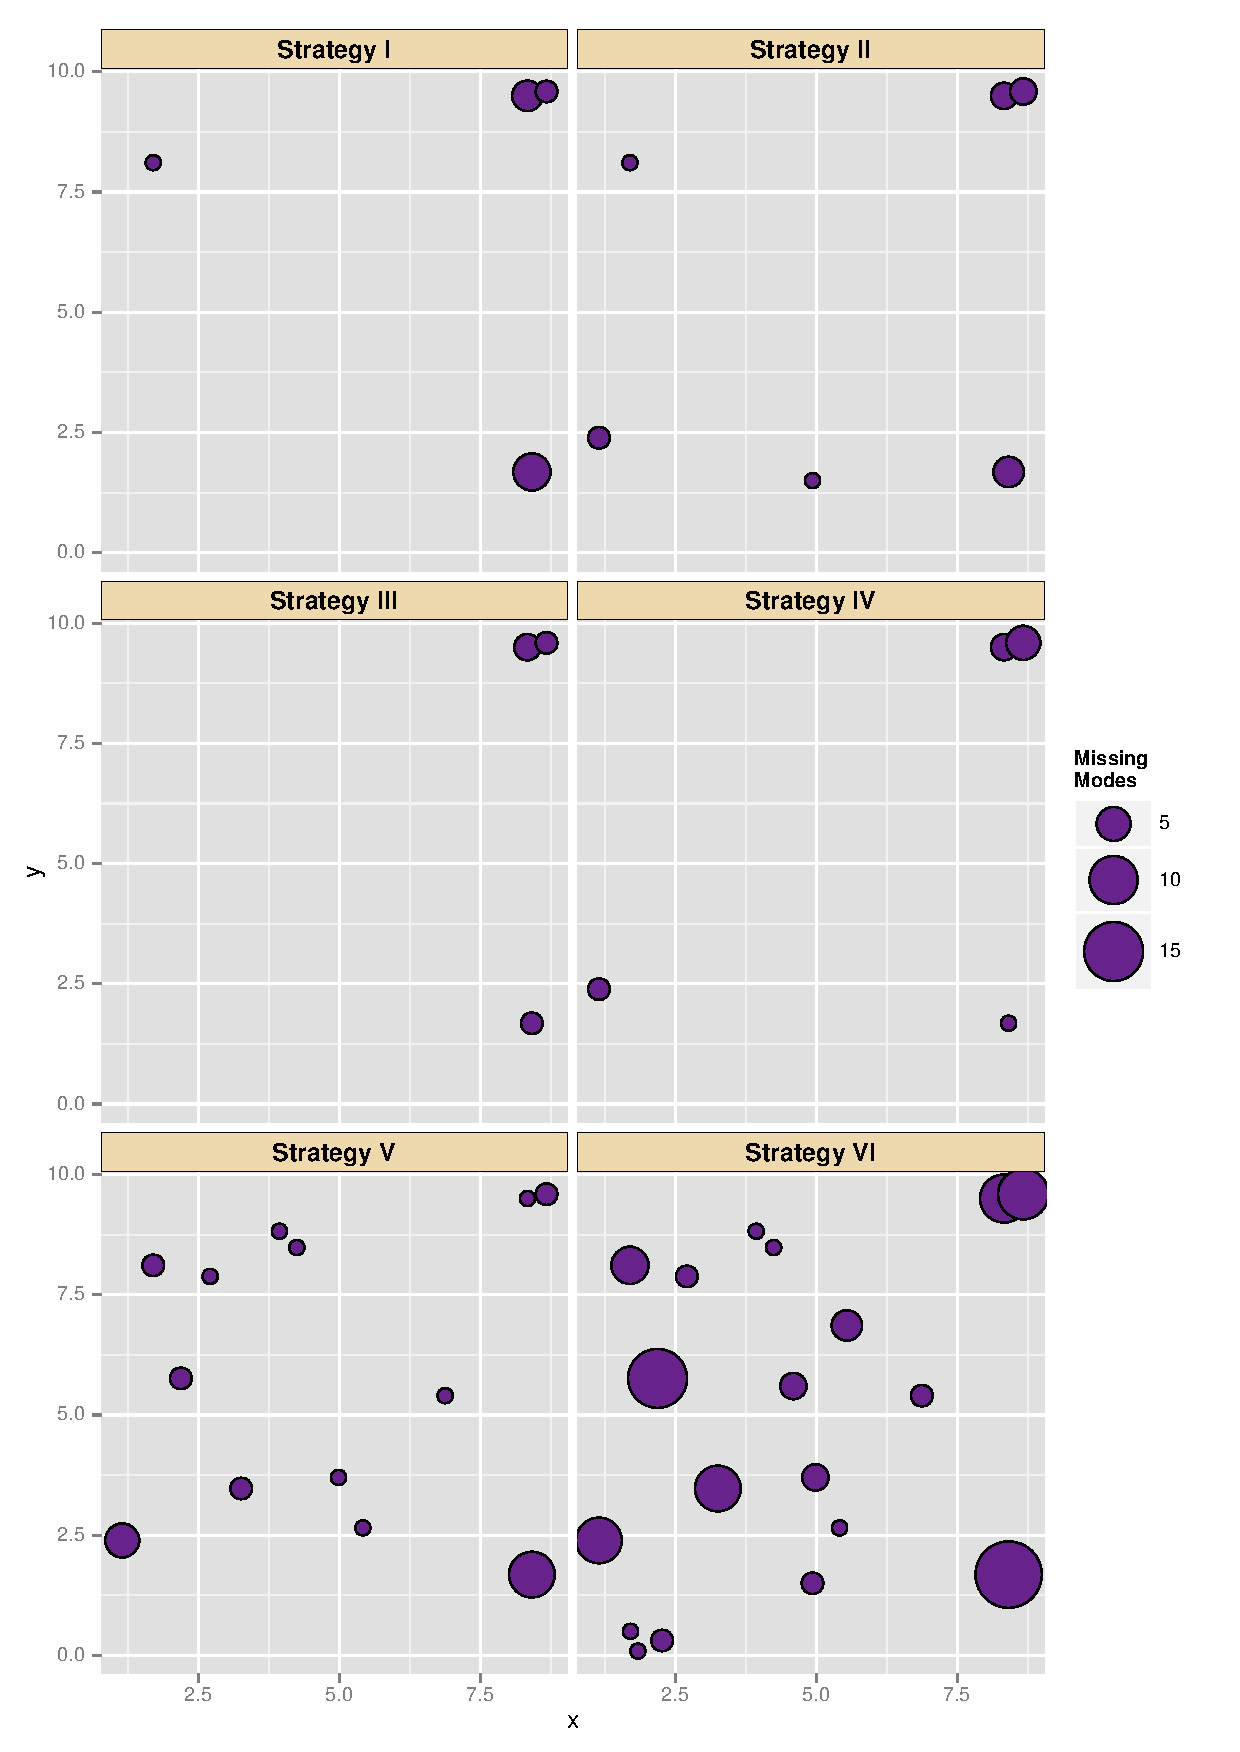
\includegraphics[height=.7\textheight,keepaspectratio=TRUE]{./img/ggplotMissingModes.pdf}
	\caption[Undiscovered Modes by the \PT\,representented by a baloon-plot.]{
		The baloon plot depicts the failure of the \PT\, under different swapping regimes to discover during one simulation all the components of the Liang's disribution, defined by Eq. \ref{againLiang}. The sample points from the simulated chains were assigned to modes using the randomised $\chi^2$-classifier. The size of the baloon corresponds to the number of simulations, out of 1000, that resulted in not assigning any points to the particular mode. The less dots appear on the plot, the more more modes were discovered, 
	}\label{missingModes}
\end{figure}

Another way of comparing different strategies is to see how they manage to approximate the weights of different modes in the entire distribution. A possible criterion for measuring the quality of approximation is to look upon the average absolute error. It averages the absolute distance of a simulation approximation of weight from the true one, equal to $0.05$. Figure \ref{AAE} summarises the results of such procedure.

What can be seen in Figure \ref{AAE} is that again the state-independent proceduters are notably worse in prescribing the correct weights to different modes. The average absolute errors reach $0.025$ and even $0.03$ which amounts to respectively $50\%$ and $60\%$ of the true value, which is much. It's worth stressing however that even the winning \ref{strat1}, that manages to score best in 18 out of 20 modes, sometimes reaches a $50\%$ relative\footnote{Again with respect to $0.05$} error. It's best result is to score a mearly $30\%$ relative error.         

\begin{figure}[ht]
	\centering 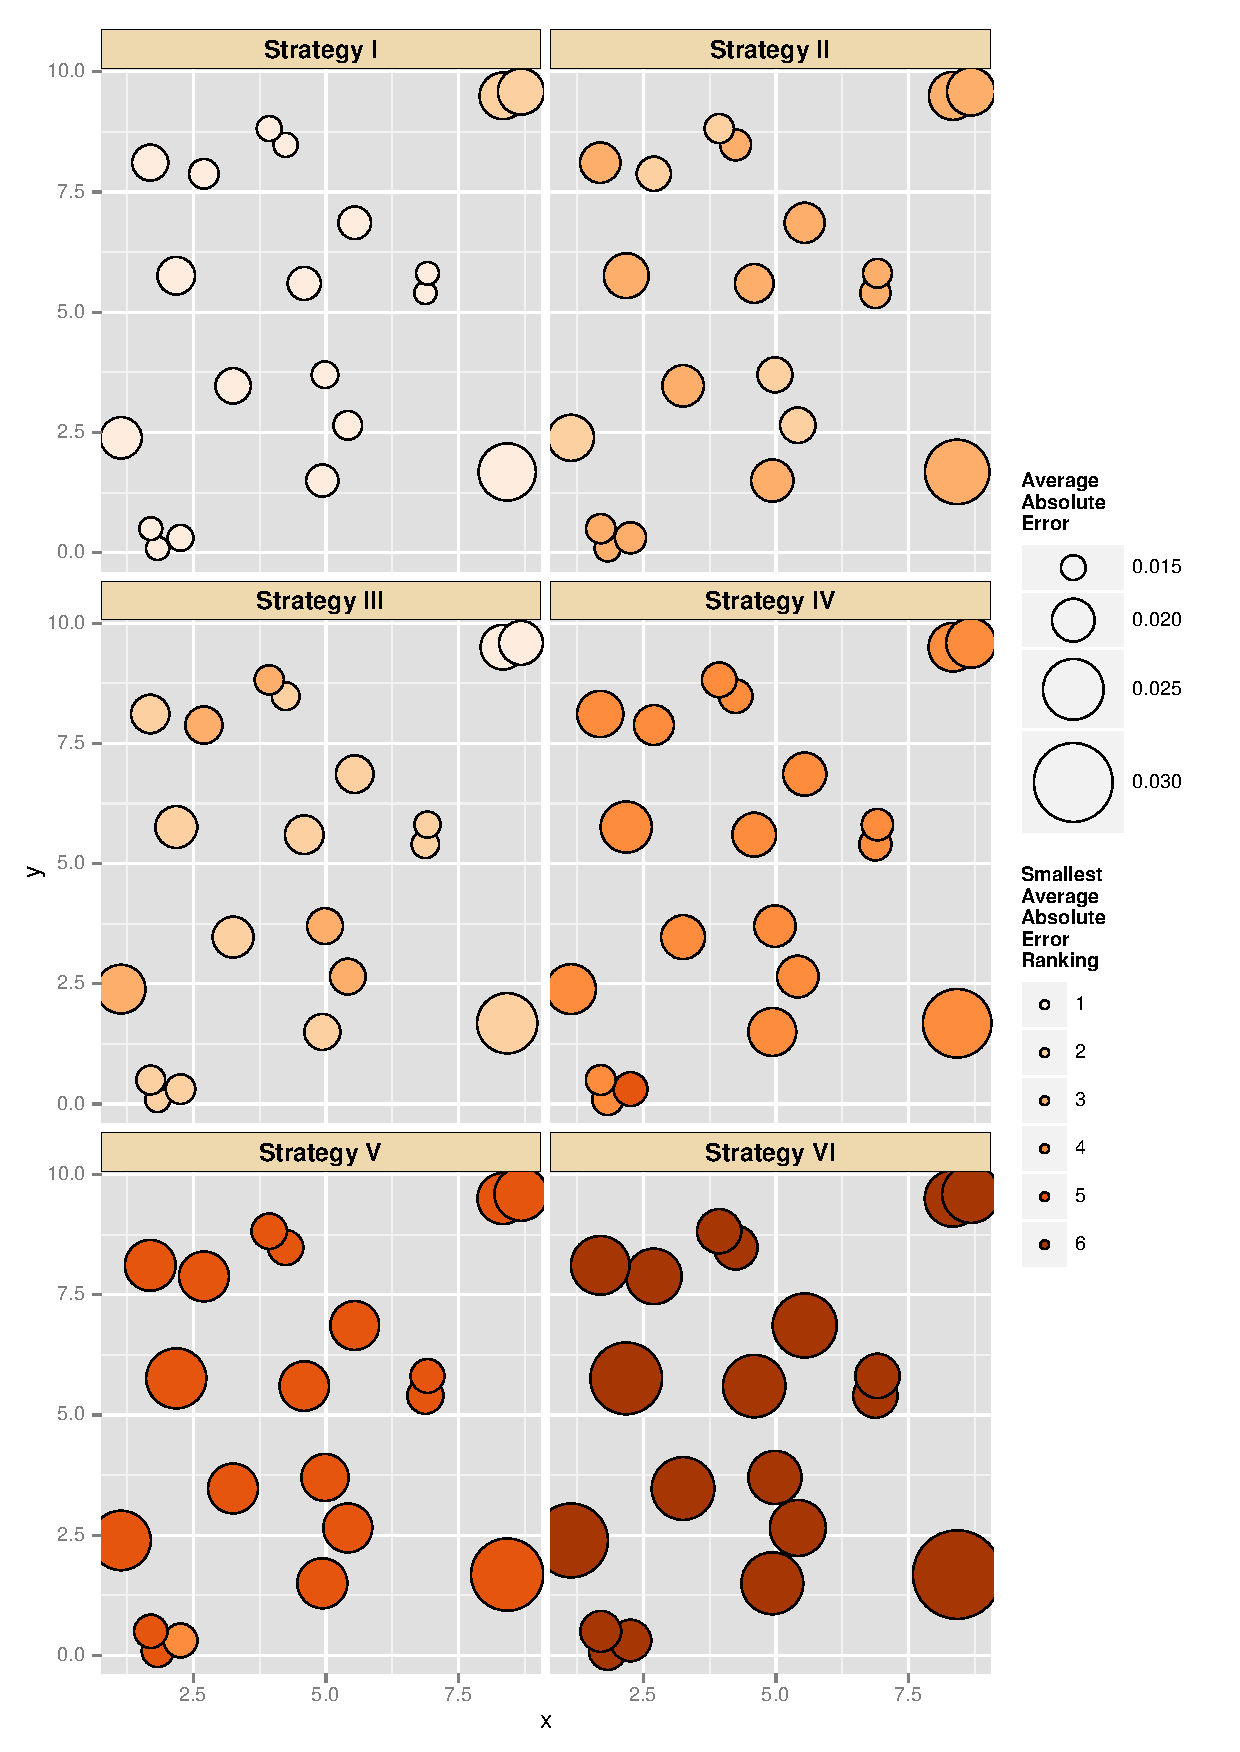
\includegraphics[height=.7\textheight,keepaspectratio=TRUE]{./img/ggplotAverageAbsoluteError.pdf}
	\caption[Average Absolute Errors in simulations consisting of 2500 iterations of the \PT.]{
		The baloon plots depicts the errors of the \PT\, in evaluating the weights of different components of the Liang's mixture, defined by Eq. \ref{againLiang}, under different Swap Strategies. The sample points from the simulated chains were assigned to modes using the randomised $\chi^2$-classifier. The error is calculated simply as the $l^1$ distance of results divided by the number of observations, being equal to 1000. It is being calculated seperately for different strategies and different distributions that compose the mixture; all of them appear with weight being equal to 0.05. The dots are coloured according to their position in the overall ranking of errors, done separately for every mode of Liang's distribution, so that the darker they are, the bigger was the error for a particular mode. The sample points from the simulated chains were assigned to modes using the randomised $\chi^2$-classifier.   
	}\label{AAE}
\end{figure}

One can also wonder whether the quality of estimates improves whith longer runs of the algorithm, that is, whether the procedure is stable and convergent. Figure \ref{shortAndLongSimulations} gives an answer to such question. All the rhombi that correspond to longer runs of the algorithm are found inside the dots that represent the shorter ones --- significantly longer runs (in the above example three times longer) do lead to overall improvement in the precision of estimates. This improvement amount to about a 50\% reduction in error, which stems from visual inspection of the length of rhombi's diagonal wiht respect to the dots' diameter. One notices also slight reshufflements in ranking among the state-dependent strategies, as in different plots pairs dot-rhombus with different colour schemes appear: \ref{strat3} seems to overtake \ref{strat2} in ranking. One can also obeserve that among the state-independent strategies there no difference in rankings, \ref{strat6} restricted to swaps between neighbouring chains loosing with \ref{strat5}. One can also notice that \ref{strat4} has better results than \ref{strat5} in one additional mode. 

\begin{figure}[ht]
	\centering 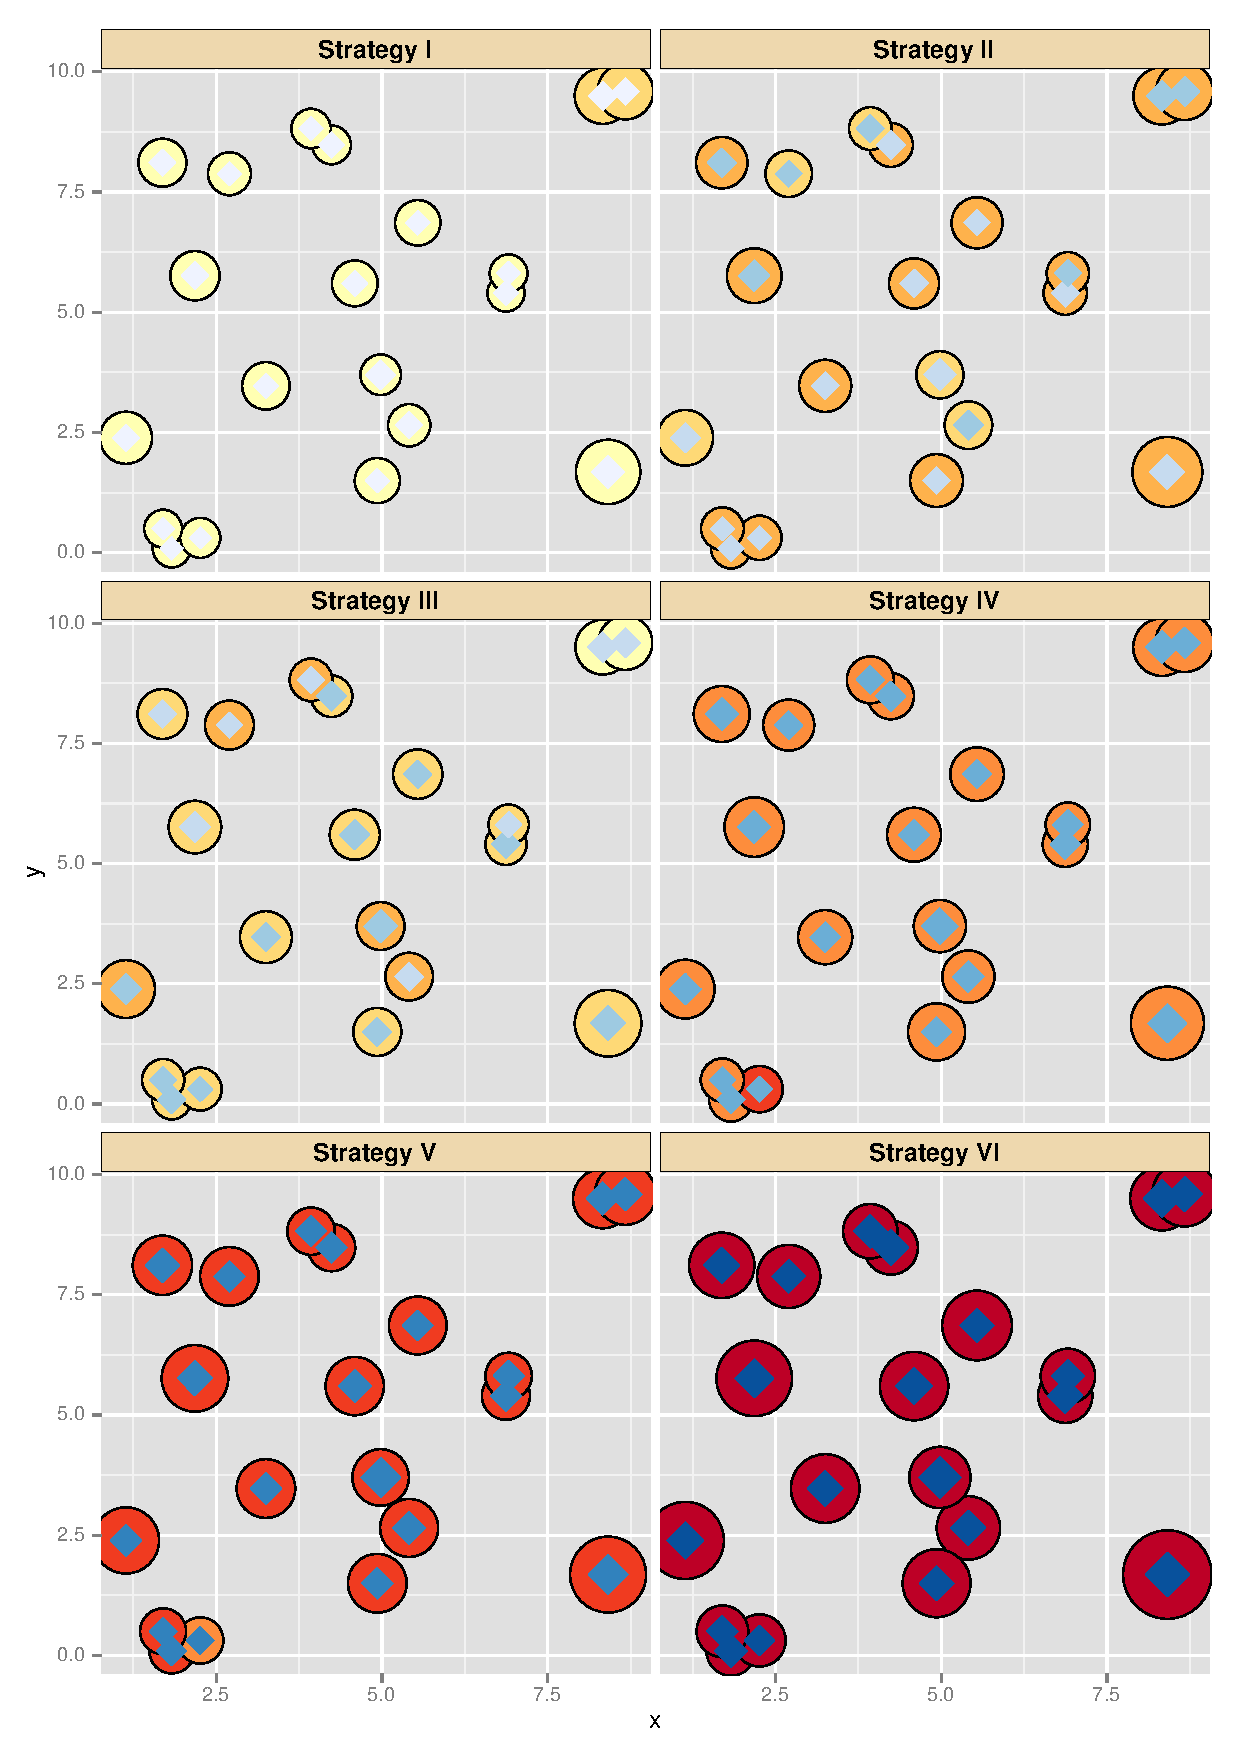
\includegraphics[height=.7\textheight,keepaspectratio=TRUE]{./img/bigSimulationOverlayed.pdf}
	\caption[Average Absolute Errors comparison between 2500 and 7500 iteration-long runs of the \PT.]{
		This figure explores the differences in the quality of the estimations of modes between shorter and longer runs of the \PT\, for different swapping strategies. Both dots and rhombi represent the Average Absolute Errors: dots correspond to shorter simulations --- 2500 iterations, and rhombi to longer simulation --- 7500 iterations, {\it ceteris paribus}. If the vertices of a given rhombus were to touch the border of a dot then errors would be the same; this, however, never occurs and the estimates are indeed much sharper. Again the colours intensity helps distinguish among the ranking of approximation: lighter colours correspond to smaller values of errors. 
	}\label{shortAndLongSimulations}
\end{figure}




One can also try to compare different strategies in their task of actually appoximating different integrals. We have restricted ourselves to evaluate how the algorithms handle the task of actually calculating the real moment of Liang's distribution. These are readily computable analytically. 

In Figure \ref{momentsBaragatti} we compare the outcomes of different Swapping Strategies in this particular task. Observe that all the strategies on average perform admiringly in this task, since the average empirical estimate of moments is very near the true value --- the rhombi are usually near the centre of the dot that marks the true value. One can see that all the algorithms better estimate the first coordinate of the mean than the second. Also the estimates of the covariance matrix show, that the variance of the $y$ coordinate have bigger variance. Within the state-independent group of strategies it is also apparent that the possibility to accept swaps from not-neighbouring chains results in a concentration of the empirical distribution. However results of state-dependent strategies seem to be fairly comparable. 

\begin{figure}
	\begin{minipage}[b]{.5\linewidth}
		\centering 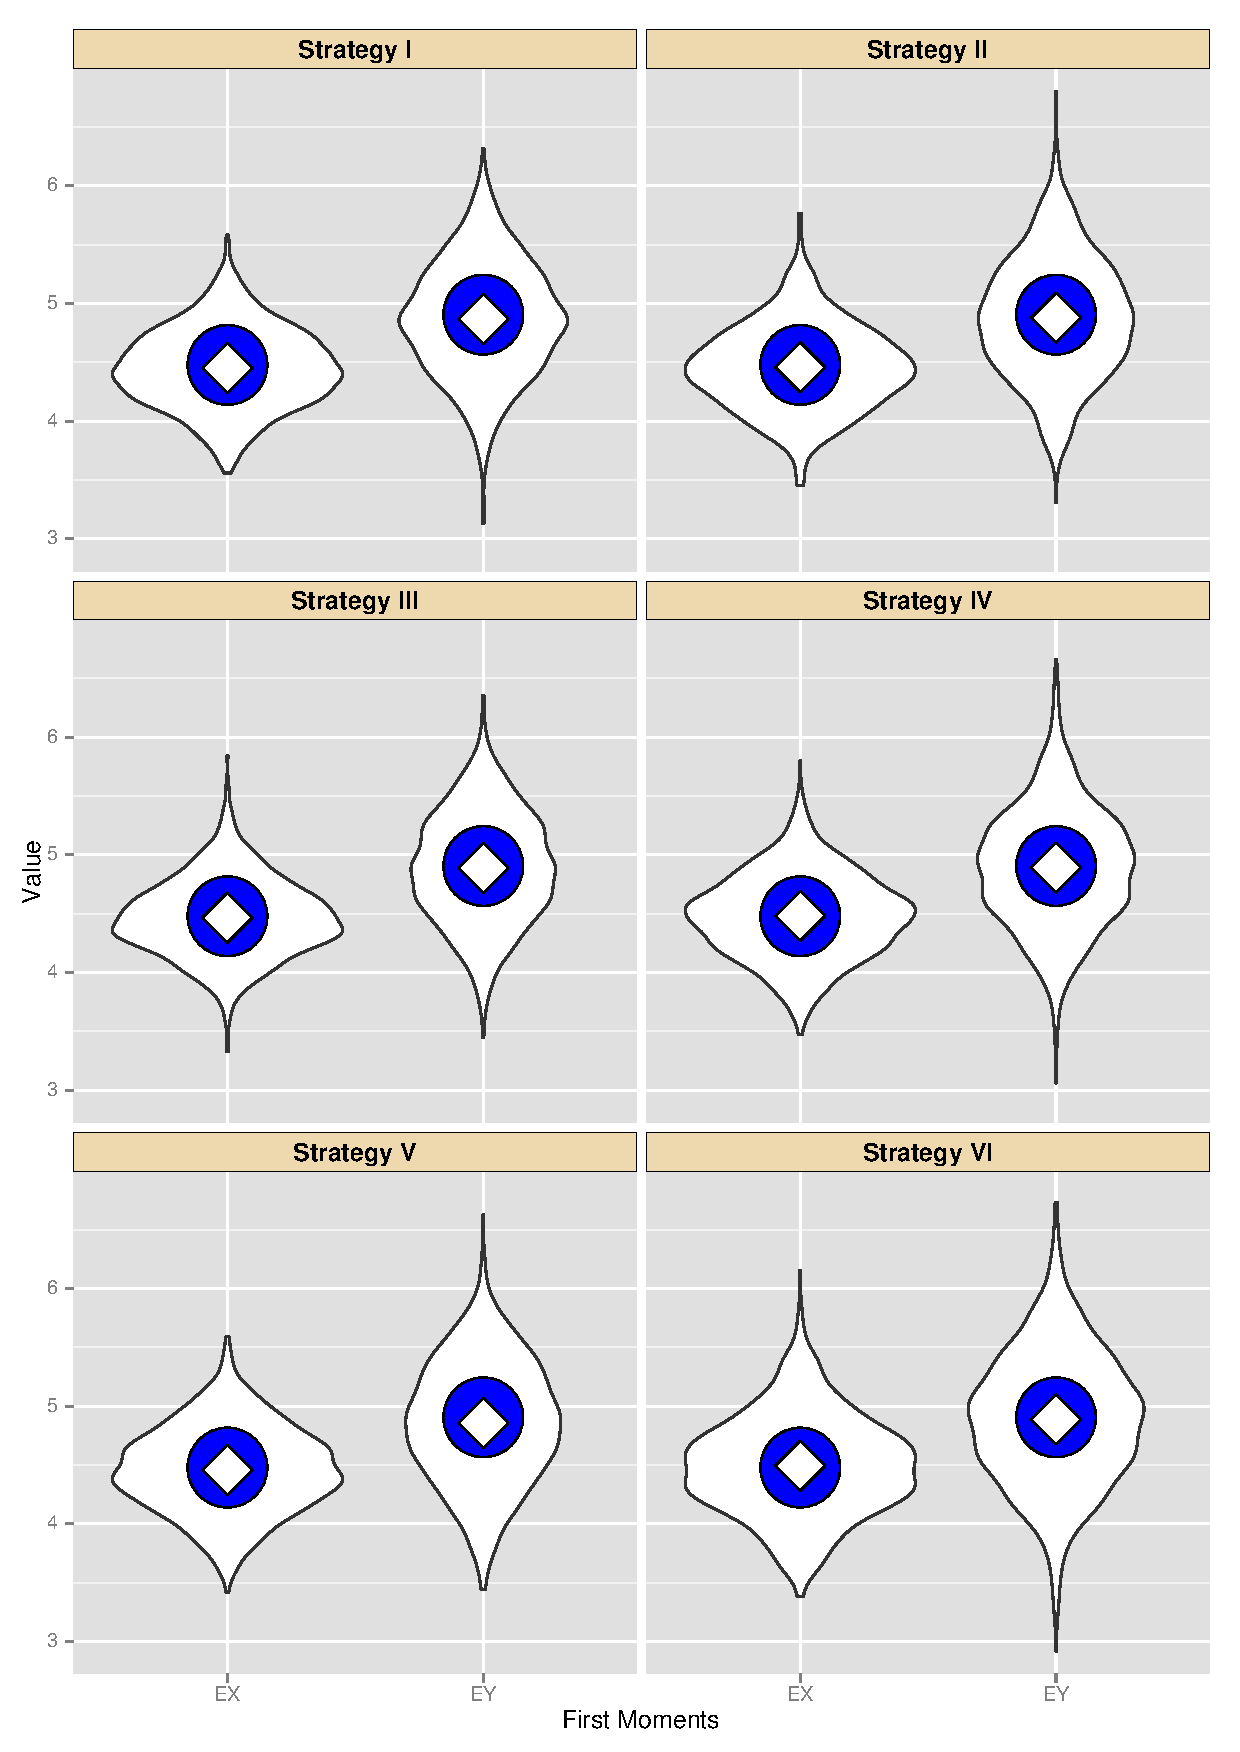
\includegraphics[width=\textwidth,keepaspectratio=TRUE]{./img/firstMomentsBaragatti.pdf}
		\subcaption{First Moments}\label{firstMomentsBaragatti}
	\end{minipage}%
	\begin{minipage}[b]{.5\linewidth}
		\centering 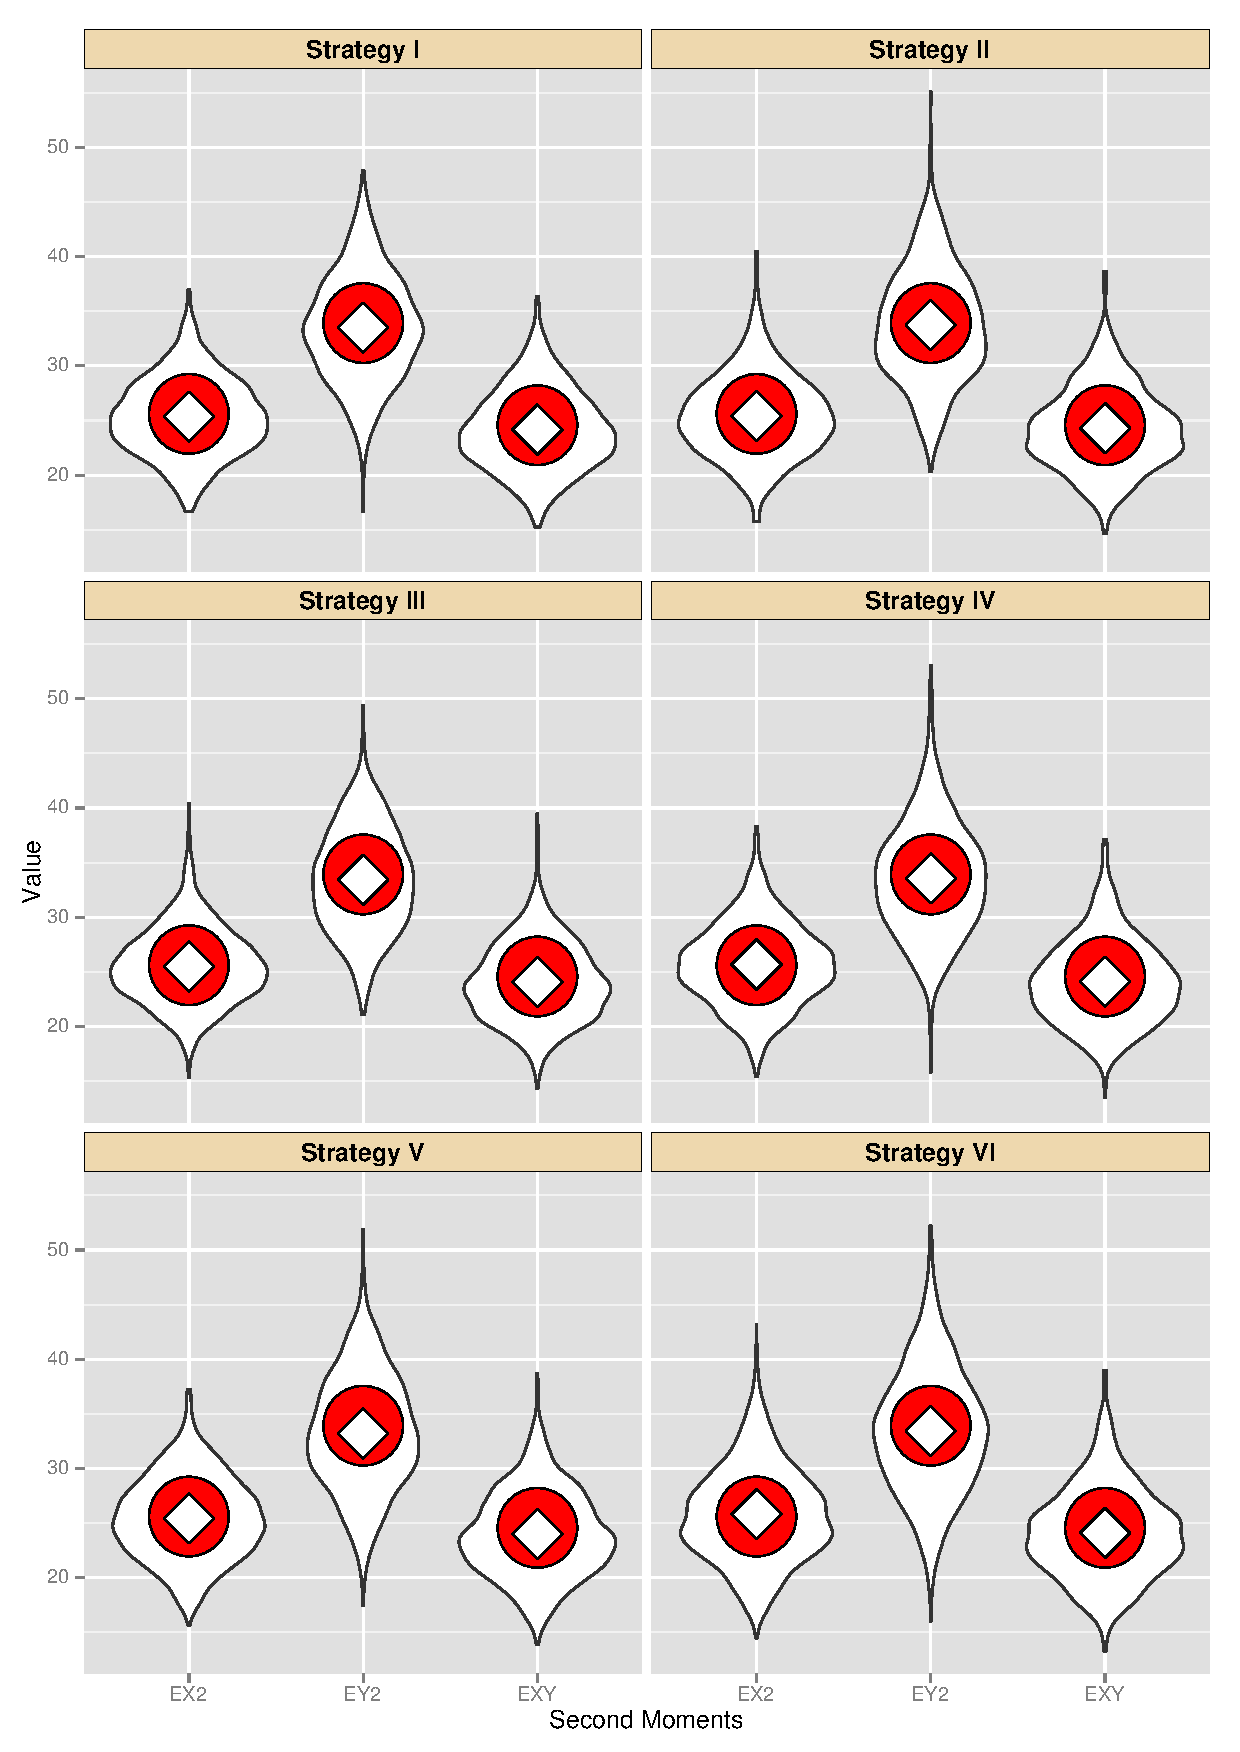
\includegraphics[width=\textwidth,keepaspectratio=TRUE]{./img/secondMomentsBaragatti.pdf}
	\subcaption{Second Moments}\label{secondMomentsBaragatti}
	\end{minipage}
	\caption[First and Second moments of the Liang Distribution approximations --- distributions represented by a violin-plot.]{
		The violin plots depict smoothened distributions of first and second moments of the Liang mixture, described by Eq. \ref{againLiang}, for different \textsc{Swap Strategies}. The empirical means are ploted as white rhombi on the blue background. The blue dots are centered at Liang Distribution's exactly calculated moments, so that one can asses the differences of theory and experiment simply by comparing the relative posititioning of the centres of rhombi and dots.
	}\label{momentsBaragatti}
\end{figure}

	\chapter*{Summary and Future Research Directions}
\addcontentsline{toc}{chapter}{Summary}

As seen in the Chapter \ref{motivation} the standard Metropolis-Hastings algorithm has intrinsic limitations when it comes to solving the \ref{Problem} of drawing sample points from multimodal distributions. The \PT\, serves as a potential solution to that \ref{Problem}, being at the same time quite a flexible approach. 

In this work we have envisaged several Swapping Strategies. These Strategies are nothing else but laws according to which the \PT\, travels through the \sspace. \ref{strat1} served together with \ref{strat5} and \ref{strat6} as reference points for the remaining three strategies. \ref{strat1} is based on the idea of \textsc{PTEEM} devised by \citet{BaragattiParallelTemperingWithEquiEnergyMoves} of swaps occuring between chains that end up having the most similar temperature levels. \ref{strat5} and \ref{strat6} on the other hand are state-independent strategies, as exposed in \citet{BM2}. Two different measures have showed a slight improvement in approximating the target distribution as measured by the two-dimensional \textsc{KS} statistics and the count of undiscovered modes when using \ref{strat3}. On the other hand the criterion based on measuring approximated Average Absolute Error\footnote{Approximated by the arbitrary but reasonable choice of the sample points classifier.} has given better results when using \ref{strat1}. However all the measures yield fairly similar results in that the state-dependent strategies are better than state-independent strategies and so their use seems more than plausible when solving real life problems. 

All the necessary calculations were done using a state-of-the-are programme written in \textbf{R} statistical computation language. The implementation envisages a meticulously applied object oriented programming paradigm dictated by the modularity of the problem, as exposed in Chapter \ref{Implementation}. The modularity of the solution to the \ref{Problem} stems from instrinsic features of the Markov Chain Monte Carlo that can be better understood by the study of its more abstract mathematical formulation that underlines the possibility of using virtually any \sspace. From the statement of this fact the observation, that both the \MH\, and the \PT\, can be understood as algorithms that need as input only evaluations of different probabilities. The probability measure\footnote{With minor exception for the Quasi-Metric applied in \ref{strat4}.} is therefore the only link between the implementation of the \sspace\, and the implementation of the \algo. 

In search for some good measure of comparing different strategies, the \textsc{KS} statistics was given appropriate attention. Because of the lack of a R-implemented software, a new implementation was derived, based on approach derived by \citet{NiVingron}, with minor improvements that prevent from unnecessary calculations.

All of the implemented software is to be shiped soon as an independent \textbf{R} package.           

As for the future plans an implementation of an adaptive version of the \PT\, is planned. The need for such algorithm stems from a potential drawback in the \PT, which is the lack of a unified approach to setting up the temperature levels. In fact the internalisation of such procedures into the algorithmic model could enhance mightly the efficiency parameters of the algorithm, e.g. by reduction in the number of unnecessary chains. 

We also think that implementation of the \textsc{KS} calculator can be significanlty improved by meticulous application of the multi-dimensional {\it divide et impera} approach, originally developed by \citet{Jon}.  

Moreover, for technical reasons the derived template should be re-implemented using a faster and more orderly computer language, such as \textbf{C++}.

	\bibliographystyle{./bibliography/eccaNoNotes}
	% \bibliography{./bibliography/myBooks}
	\bibliography{myBooks}

\end{document}






%%% Przydatne

\begin{figure}
	\begin{minipage}[b]{.5\linewidth}
		\centering 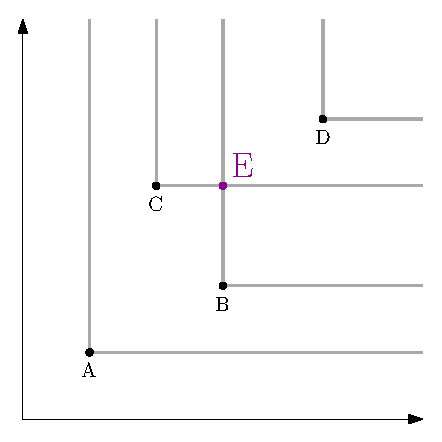
\includegraphics[scale=1]{./img/KS1.eps}
		\subcaption{Sample points and level sets of an examplary \ecdf.}\label{simpleEcdf}
	\end{minipage}%
	\begin{minipage}[b]{.5\linewidth}
		\centering 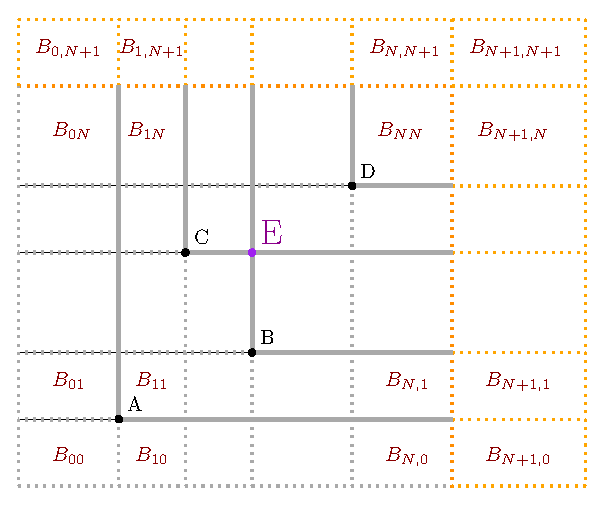
\includegraphics[scale=1]{./img/KS2.eps}
	\subcaption{Division of the state-space.}\label{fig:1b}
	\end{minipage}
	\caption{Calculations of the KS-distance.}\label{fig:1}
\end{figure}
s
The applicability of the PT algorithm in molecular biology stems mostly from the ever growing interest in the Bayesian inference. The mixture models for instance have been applied in the identification of gene co-expression patterns in microarray data. With the spread of use of such methods, the PT algorithm gains of importance.